\documentclass[12pt]{aghdpl}
% \documentclass[en,11pt]{aghdpl}  % praca w języku angielskim

% Lista wszystkich języków stanowiących języki pozycji bibliograficznych użytych w pracy.
% (Zgodnie z zasadami tworzenia bibliografii każda pozycja powinna zostać utworzona zgodnie z zasadami języka, w którym dana publikacja została napisana.)
\usepackage[english,polish]{babel}

% Użyj polskiego łamania wyrazów (zamiast domyślnego angielskiego).
\usepackage{polski}

\usepackage[utf8]{inputenc}

% dodatkowe pakiety
\usepackage{float}			%added to position tables inline
%\restylefloat{table}		
\usepackage{mathtools}
\usepackage{amsfonts}
\usepackage{amsmath}
\usepackage{amsthm}
\usepackage{textcomp}		%added for degree symbol
\usepackage{hyperref}		%added for clickable references
\usepackage[table]{xcolor}	%added for coloring cells
%\usepackage{url}			%added for URLs in bibliography

% --- < bibliografia > ---

\usepackage[
style=numeric,
sorting=none,
%
% Zastosuj styl wpisu bibliograficznego właściwy językowi publikacji.
language=autobib,
autolang=other,
% Zapisuj datę dostępu do strony WWW w formacie RRRR-MM-DD.
urldate=iso8601,
% Nie dodawaj numerów stron, na których występuje cytowanie.
backref=false,
% Podawaj ISBN.
isbn=true,
% Nie podawaj URL-i, o ile nie jest to konieczne.
url=false,
%
% Ustawienia związane z polskimi normami dla bibliografii.
maxbibnames=3,
% Jeżeli używamy BibTeXa:
backend=bibtex
]{biblatex}

\usepackage{csquotes}
% Ponieważ `csquotes` nie posiada polskiego stylu, można skorzystać z mocno zbliżonego stylu chorwackiego.
\DeclareQuoteAlias{croatian}{polish}

\addbibresource{bibliografia.bib}

% Nie wyświetlaj wybranych pól.
%\AtEveryBibitem{\clearfield{note}}


% ------------------------
% --- < listingi > ---

% Użyj czcionki kroju Courier.
\usepackage{courier}

\usepackage{listings}
\lstloadlanguages{TeX}

\lstset{
	literate={ą}{{\k{a}}}1
	{ć}{{\'c}}1
	{ę}{{\k{e}}}1
	{ó}{{\'o}}1
	{ń}{{\'n}}1
	{ł}{{\l{}}}1
	{ś}{{\'s}}1
	{ź}{{\'z}}1
	{ż}{{\.z}}1
	{Ą}{{\k{A}}}1
	{Ć}{{\'C}}1
	{Ę}{{\k{E}}}1
	{Ó}{{\'O}}1
	{Ń}{{\'N}}1
	{Ł}{{\L{}}}1
	{Ś}{{\'S}}1
	{Ź}{{\'Z}}1
	{Ż}{{\.Z}}1,
	basicstyle=\footnotesize\ttfamily,
}

% ------------------------

\AtBeginDocument{
	\renewcommand{\tablename}{Tabela}
	\renewcommand{\figurename}{Rys.}
}

% ------------------------
% --- < tabele > ---

\usepackage{array}
\usepackage{tabularx}
\usepackage{multirow}
\usepackage{booktabs}
\usepackage{makecell}
\usepackage[flushleft]{threeparttable}

% defines the X column to use m (\parbox[c]) instead of p (`parbox[t]`)
\newcolumntype{C}[1]{>{\hsize=#1\hsize\centering\arraybackslash}X}


%---------------------------------------------------------------------------

\author{Piotr Ziębiński}
\shortauthor{P. Ziębiński}

%\titlePL{Przygotowanie bardzo długiej i pasjonującej pracy dyplomowej w~systemie~\LaTeX}
%\titleEN{Preparation of a very long and fascinating bachelor or master thesis in \LaTeX}

\titlePL{Układ do tłumienia zakłóceń z otoczenia}
\titleEN{Circuit for surrounding noise cancellation}

\shorttitlePL{Układ do tłumienia zakłóceń z otoczenia} % skrócona wersja tytułu jeśli jest bardzo długi
\shorttitleEN{Circuit for surrounding noise cancellation}

\thesistype{Praca dyplomowa inżynierska}
%\thesistype{Master of Science Thesis}

\supervisor{dr hab. inż. Krzysztof Kasiński}
%\supervisor{Marcin Szpyrka PhD, DSc}

\degreeprogramme{Mikroelektronika w Technice i Medycynie}
%\degreeprogramme{Computer Science}

\date{2019}

\department{Katedra Metrologii i Elektroniki}
%\department{Department of Applied Computer Science}

\faculty{Wydział Elektrotechniki, Automatyki,\protect\\[-1mm] Informatyki i Inżynierii Biomedycznej}
%\faculty{Faculty of Electrical Engineering, Automatics, Computer Science and Biomedical Engineering}

\acknowledgements{Serdecznie dziękuję mojemu promotorowi za pomoc i podpowiedzi przy tworzeniu pracy}

\setlength{\cftsecnumwidth}{10mm}

%---------------------------------------------------------------------------
\setcounter{secnumdepth}{4}
\brokenpenalty=10000\relax

\begin{document}
	
	\titlepages
	
	% Ponowne zdefiniowanie stylu `plain`, aby usunąć numer strony z pierwszej strony spisu treści i poszczególnych rozdziałów.
	\fancypagestyle{plain}
	{
		% Usuń nagłówek i stopkę
		\fancyhf{}
		% Usuń linie.
		\renewcommand{\headrulewidth}{0pt}
		\renewcommand{\footrulewidth}{0pt}
	}
	
	\setcounter{tocdepth}{2}
	\tableofcontents
	\clearpage
	\raggedbottom 
	\chapter{Wstęp}
\label{cha:wstep}

Otaczający nas świat jest pełen dźwięków pochodzących z różnych źródeł. Możemy wyróżnić dźwięki powszechnie uważane za przyjemne dla ucha, jak ćwierkanie ptaków oraz te nieprzyjemne jak dźwięk wiercenia. Narażenie na nadmierny hałas jest w dużej mierze zależne od naszego miejsca pracy. Pracownika biurowego będą irytować samochody słyszane przez uchylone okno, a dla robotnika pracującego przy kładzeniu asfaltu ruchliwa droga to normalny dźwięk otoczenia. Ze względu na charakter pracy, w poziom dźwięku w pomieszczeniach biurowych reguluje polska norma "Dopuszczalne wartości poziomu dźwięku na stanowisku pracy"\cite{PolskaNormaCisnienia}. Mimo to obaj pracownicy są równie narażeni na skutki przebywania w ciągłym hałasie.

Wystawienie na zbyt wysoki poziom ciśnienia akustycznego prowadzi do rozdrażnienia, zmęczenia, a w konsekwencji do uszkodzenia słuchu. Z tego powodu tworzone są różne rozwiązania pozwalające polepszyć samopoczucie i chronić słuch. 

Fala akustyczna jest falą mechaniczną, dlatego można ją stosunkowo łatwo tłumić bez użycia elektroniki. Takie rozwiązanie ma jednak swoje wady. Słuchawka musi być duża i ciężka, żeby zmieścić jak najwięcej materiału tłumiącego, a sama metoda działa dobrze dla częstotliwości od 20Hz do 800Hz i tłumi do 30dB\cite{SennheiserANC}. Z pomocą przychodzą układy elektroniczne służące do aktywnego tłumienia zakłóceń, czyli nakładania fali przesuniętej w fazie o 180\textdegree\ na oryginalny dźwięk. Te z kolei dzielą się na cyfrowe oraz analogowe. Różnica polega na tym, że pierwsze oprócz innych elementów, jak wzmacniacze, korzystają też z przetworników i algorytmów do przetwarzania sygnałów.

Praktyczne zastosowania różnych technik tłumienia fal akustycznych można wymieniać bez końca. Są to między innymi:
\begin{itemize}
	\item przydrożne ekrany dźwiękochłonne
	\item ochronniki słuchu ogólnego zastosowania
	\item słuchawki multimedialne z ANC (ang. \textit{Active Noise Cancelling} - Aktywne Tłumienie Szumu)
	\item systemy wyciszania w pojazdach
	\item strzeleckie ochronniki słuchu
\end{itemize}

W mojej pracy skupiłem się na tych ostatnich. Postanowiłem zaprojektować, zaprogramować i zbudować słuchawki taktyczne, które w normalnych warunkach przepuszczają dźwięki z zewnątrz i umożliwiają normalny odbiór dźwięków otoczenia, a w razie wystąpienia niebezpiecznie dużych natężeń - wytłumiają aktywnie, chroniąc słuch.
	
	\chapter{Dźwięk}
\label{cha:dwiek}

\section{Ogólna charakterystyka fal dźwiękowych}
Dźwięk jest wrażeniem słuchowym, powodowanym przez fale akustyczne. Rozchodzą się one w postaci fal podłużnych, będącymi zaburzeniami ciśnienia i gęstości ośrodka sprężystego\cite{FaleAkustyczne}. Prędkość dźwięku w powietrzu przy temperaturze 0 stopni celciusza wynosi 331,3m/s.

Dźwięk można opisać kilkoma podstawowymi parametrami:

\begin{itemize}
	\item wysokość (częstotliwość fali)
	\item głośność (amplituda fali)
	\item barwa (skład widmowy)
	\item czas trwania
\end{itemize}

Poziom dźwięku wyrażany jest miarą ciśnienia akustycznego, którego jednostką jest Paskal \textit{Pa}. Jednak ponieważ ludzkie ucho reaguje na bodźce logarytmicznie, częściej używa się decybeli ($\frac{1}{10}$ bela). Wzór na obliczenie poziomu ciśnienia akustycznego w skali logarytmicznej wygląda następująco\cite{CisnienieAkustyczne}:
\begin{equation}
SPL = 20\log{(\frac{p}{p_{ref}})}
\end{equation}

gdzie: \\
\indent$SPL$ - poziom ciśnienia akustycznego [\textit{dB}], \\
\indent$p$ - ciśnienie akustyczne [\textit{Pa}], \\
\indent$p_{ref}$ - ciśnienie akustyczne odniesienia, czyli próg słyszalności, wynoszący $2\cdot10^{-5} Pa$ 


\section{Odbiór fal dźwiękowych przez człowieka}
W ludzkim uchu odbiór dźwięku odbywa się przez zmiany ciśnienia płynu, którym wypełniony jest ślimak (patrz rys. \ref{slimak}). Powodują one podrażnianie rzęsek, które z kolei przekazują impulsy elektrochemiczne do mózgu. Im mniejsza częstotliwość fali, tym dalej ona dociera i na tej podstawie mózg potrafi rozróżniać częstotliwości. Dla człowieka słyszalne są fale z zakresu ok. 20Hz - 20kHz, choć górna granica maleje z wiekiem przez stopniową degradację najbardziej zewnętrznych rzęsek (a więc odpowiadających za najwyższe częstotliwości)\cite{JakSlyszymy}. 
Fale poniżej granicy słyszalności to infradźwięki, powyżej - ultradźwięki, a częstotliwości wyższe, niż $10^{10}kHz$ to hiperdźwięki.

\begin{figure}[H]
	\centering
	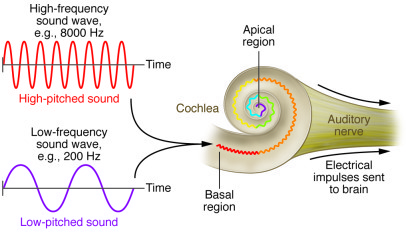
\includegraphics{zdjecia/slimak.png}
	\caption{\label{slimak} Odbiór fal dźwiękowych w ślimaku ludzkiego ucha\cite{cochlea}}
\end{figure}


\section{Fale dźwiękowe jako zagrożenie dla zdrowia człowieka}

Głównym, choć nie jedynym, parametrem dźwięku, który determinuje jego szkodliwość jest amplituda fali, czyli ciśnienie akustyczne. W tabeli \ref{tab:SPL} przedstawiono sytuacje, w których występuje określony poziom natężenia.

\begin{table}[H]
	\centering
	\begin{tabular}{|r|l|}
		\hline
		Natężenie [dB] & Sytuacja \\
		\hline
		\hline
		\rowcolor{red!50}
		130 & Młot pneumatyczny \\
		\hline
		\rowcolor{red!40}
		120 & Klakson z odległości 1m \\
		\hline
		\rowcolor{red!30}
		110 & Lotnisko \\
		\hline
		\rowcolor{red!20}
		100 & Przejazd pociągu \\
		\hline
		\rowcolor{orange!20}
		90 & Wnętrze autobusu \\
		\hline
		\rowcolor{yellow!20}
		80 & Zatłoczona ulica \\
		\hline
		\rowcolor{green!30}
		70 & Konwersacja \\
		\hline
		\rowcolor{green!30}
		60 & Salon z cichą muzyką \\
		\hline
		\rowcolor{green!30}
		50 & Biuro \\
		\hline
		\rowcolor{green!30}
		40 & Sypialnia \\
		\hline
		\rowcolor{green!30}
		30 & Studio nagraniowe \\
		\hline
		\rowcolor{green!30}
		20 & Studio radiowe \\
		\hline
	\end{tabular}
	\caption{Poziomy natężenia dźwięku\cite{SPLtable}}
	\label{tab:SPL}
\end{table}

Na szkodliwość dźwięku wpływa również czas jego trwania. Amerykańska agencja federalna NIOSH (ang. \textit{National Institute for Occupational Safety and Health}) zajmuje się badaniem i zapobieganiem chorobom związanym z pracą. Wydała ona dokument\cite{NIOSH}, w którym przedstawiono bezpieczny czas wystawienia na określone poziomy ciśnienia akustycznego\cite{SPLtable}.

\begin{table}[H]
	\centering
	\begin{tabular}{|r|l|}
		\hline
		Natężenie [dB] & Maks. czas [h] \\
		\hline
		\hline
		127 & 00:00:01 \\
		\hline
		118 & 00:00:14 \\
		\hline
		109 & 00:01:53 \\
		\hline
		100 & 00:15:00 \\
		\hline
		91 & 02:00:00 \\
		\hline
		82 & 16:00:00 \\
		\hline
	\end{tabular}
	\caption{Maksymalny czas wystawienia na określone poziomy natężęnia}
	\label{tab:SPLczas}
\end{table}

Odbiorcze uszkodzenie słuchu przez hałas nazywamy urazem akustycznym. Dzieli się go na ostry oraz przewlekły. Ostry jest powodowany krótkotrwałym oddziaływaniem natężenia powyżej 130dB, a przewlekły długotrwałym wystawieniem na dźwięki powyżej 85dB. W przypadku tego pierwszego uszkodzeniu ulega narzędzie Cortiego, będące częścią ślimaka i zawierające komórki rzęsate\cite{UrazyAkustyczne}.

\begin{figure}[H]
	\centering
	\begin{subfigure}{.45\textwidth}
		\centering
		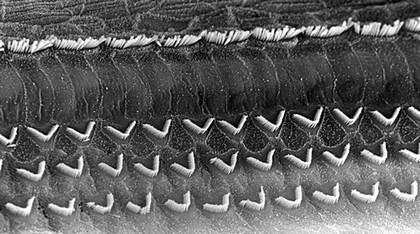
\includegraphics[scale=0.45]{zdjecia/cochlee-normale.jpg}
		\label{normal_cochlea}
		\caption{Zdrowe rzęski}
	\end{subfigure}
	\begin{subfigure}{.45\textwidth}
		\centering
		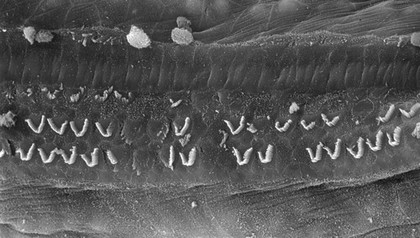
\includegraphics[scale=0.44]{zdjecia/traumatisme-sonore-niveau-2.jpg}
		\label{damaged_cochlea}
		\caption{Uszkodzone rzęski}
	\end{subfigure}
	\caption{Powierzchnia ślimaka widoczna pod mikroskopem elektronowym\cite{RzeskiMikorskop}}
\end{figure}


\subsection{Dźwięki strzałów i wybuchów}

W trakcie rozważań szczególną uwagę poświęcono dźwiękom pochodzącym od broni palnej. To właśnie one miały być głównym źródłem zagrożenia dla słuchu użytkownika. 
Ich źródłem jest eksplozja prochu strzelniczego, zmagazynowanego w łusce naboju, która nadaje prędkość początkową pociskowi. Ciśnienie akustyczne podczas takiego wybuchu przekracza $ 140 dB $, a więc wystarczy niecała sekunda, aby doprowadzić do uszkodzenia słuchu\ref{tab:SPLczas}. Dodatkowo na takie uszkodzenie najbardziej narażone są rzęski odpowiedzialne za częstotliwości między $ 3 $ a $ 6kHz $\cite{BadaniePolicjantow}. 

Aby sprawdzić częstotliwości wystrzałów różnych typów broni, zaimplementowany został program w \textit{Pythonie} do analizy dźwięków z plików \textit{.wav}. Miał on za zadanie odczytać przebieg sygnału z pliku, odfiltrować częstotliwości powyżej $ 15kHz $ i przeprowadzić szybką transformatę Fouriera na odfiltrowanym sygnale. Kod źródłowy dostępny jest na repozytorium pod linkiem \url{https://github.com/Hoplophile/Tactical_Headphones_Sim.git}. 

Schemat działania programu wygląda następująco:

\begin{figure}[H]
	\centering
	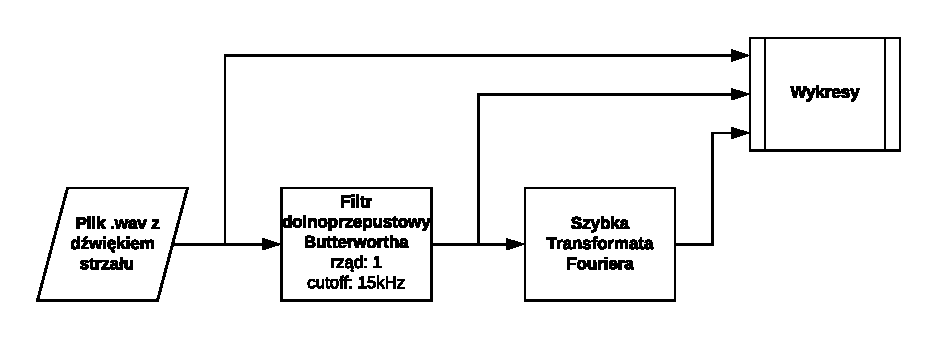
\includegraphics[scale=1]{grafy/Python_analiza_FFT.pdf}
	\caption{\label{graf:analizaFFT} Dataflow programu do analizy FFT}
\end{figure}

Pliki źródłowe z dźwiękami broni zostały pobrane ze strony \url{http://soundbible.com/tags-gun.html}. To powodowało brak pewności, czy dźwięk faktycznie pochodzi od broni podanej w nazwie oraz brak powtarzalności dźwięków, które nagrywane były w innych środowiskach, nieznanej odległości od broni i mikrofonami o różnych parametrach. Było to jednak najlepsze dostępne źródło tego typu nagrań. Wybrane zostały 4 pliki podpisane następującymi typami broni:

\begin{itemize}
	\item \textbf{M4A1} - karabin szturmowy kalibru 5.56mm
	\item \textbf{AK-47} - karabin szturmowy kalibru 7.62mm
	\item \textbf{Beretta M92} - pistolet kalibru 9mm
	\item \textbf{Mossberg 500} - strzelba (kaliber nieznany)
\end{itemize}

Program zwracał osobne wykresy dla każdego pliku źródłowego przedstawione poniżej.

\begin{figure}[H]
	\centering
	\begin{subfigure}{.49\textwidth}
		\centering
		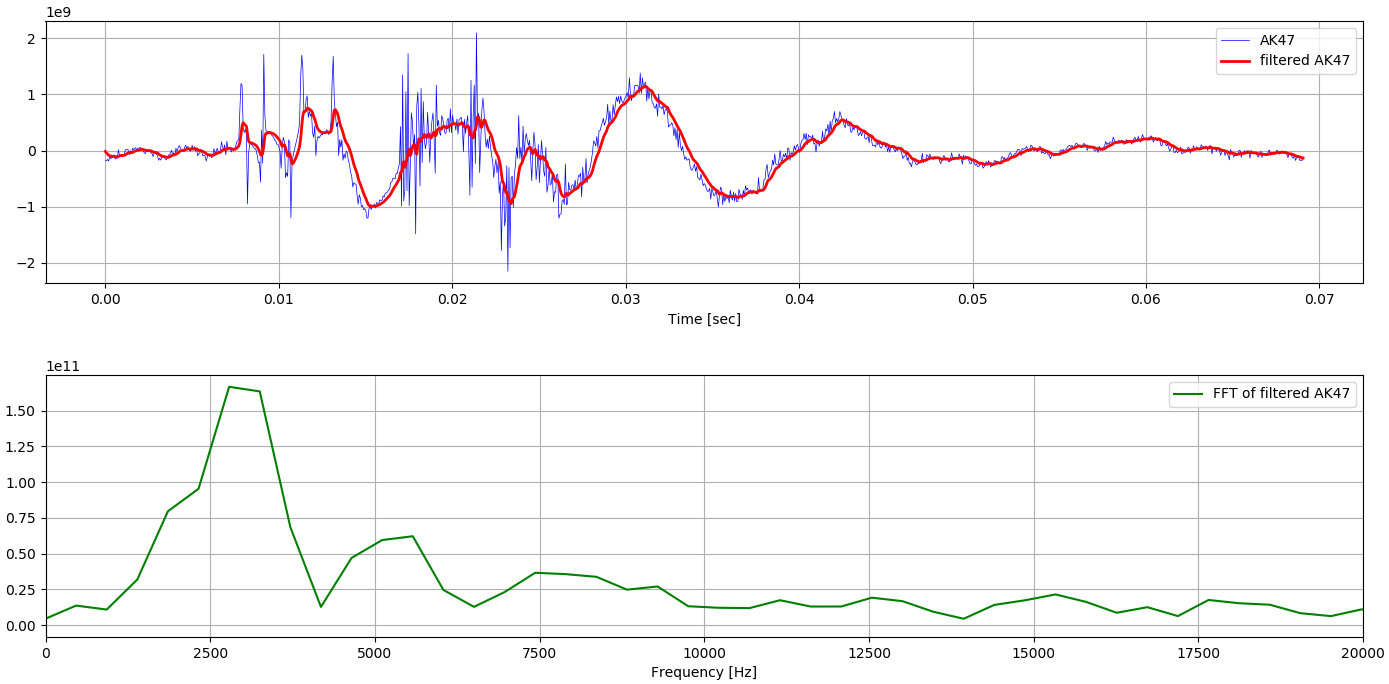
\includegraphics[height=3.9cm]{wykresy/AK47_fft.png}
		\subcaption{AK-47}
	\end{subfigure}
	\begin{subfigure}{.49\textwidth}
		\centering
		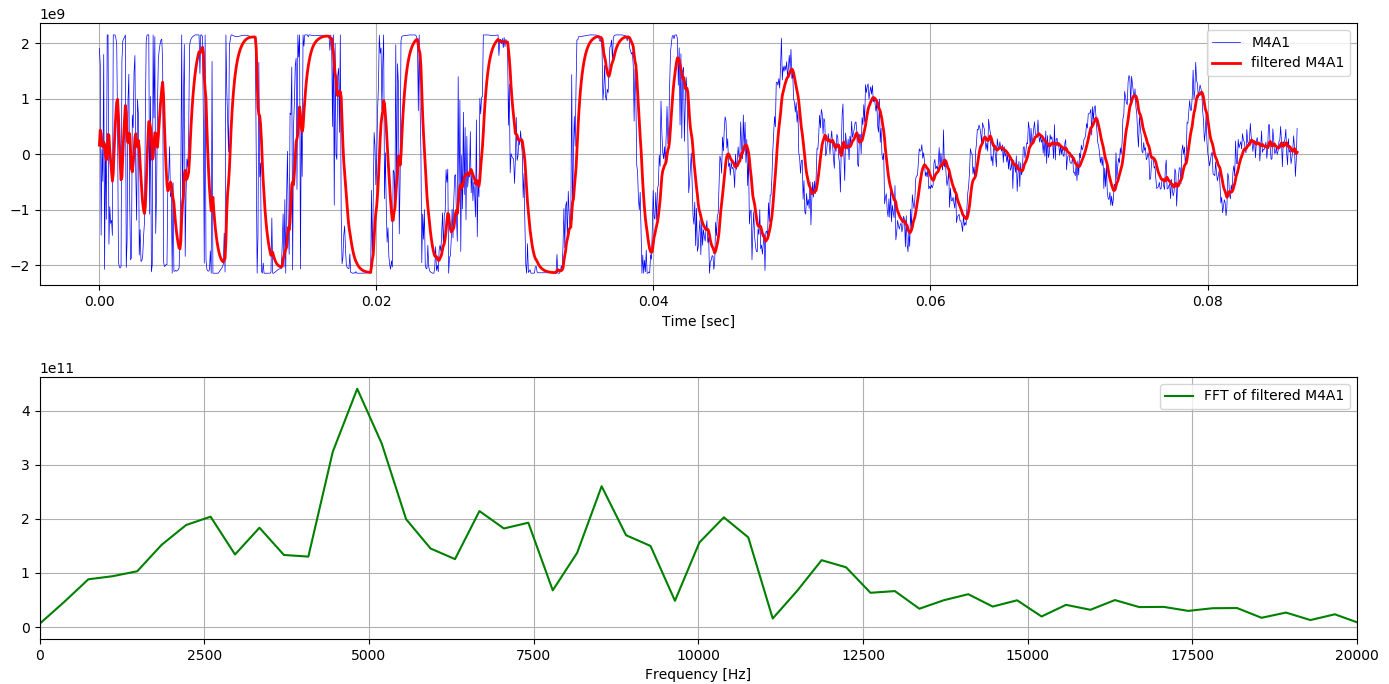
\includegraphics[height=3.9cm]{wykresy/M4A1_fft.png}
		\subcaption{M4A1}
	\end{subfigure}
	\begin{subfigure}{.49\textwidth}
		\centering
		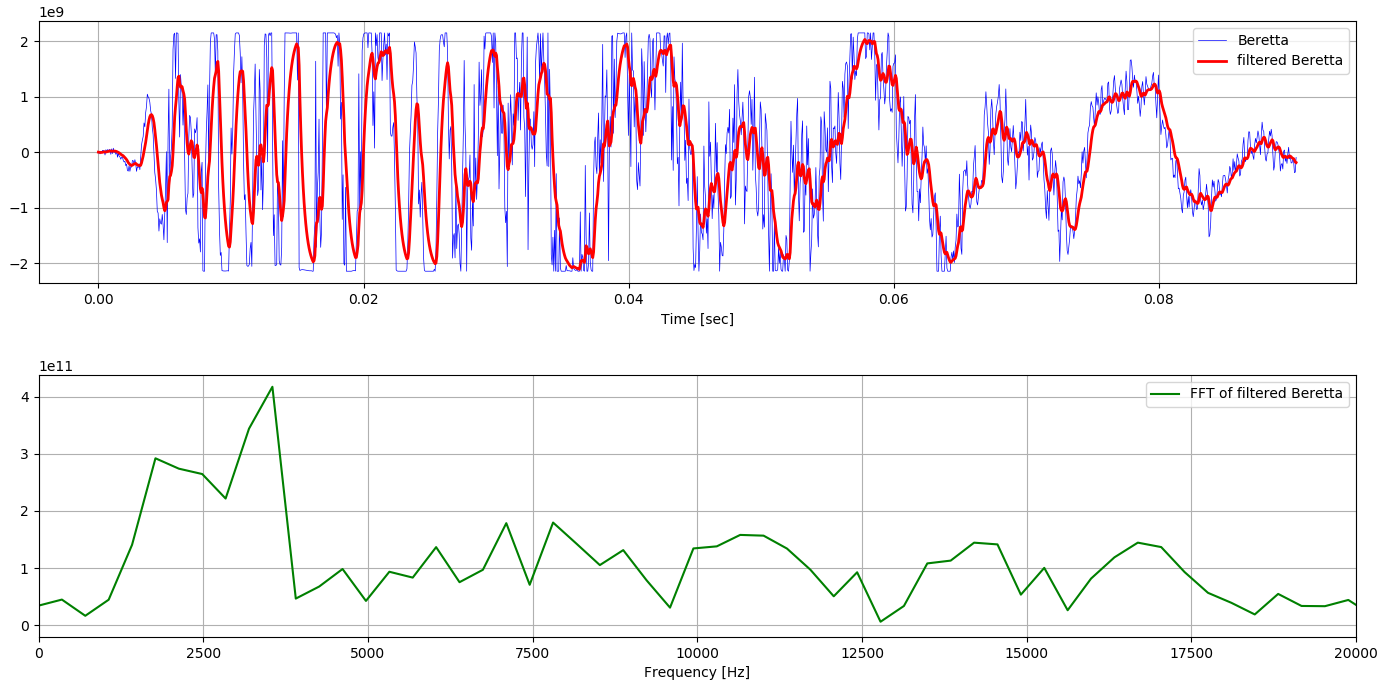
\includegraphics[height=3.9cm]{wykresy/Beretta_fft.png}
		\subcaption{Beretta M92}
	\end{subfigure}
	\begin{subfigure}{.49\textwidth}
		\centering
		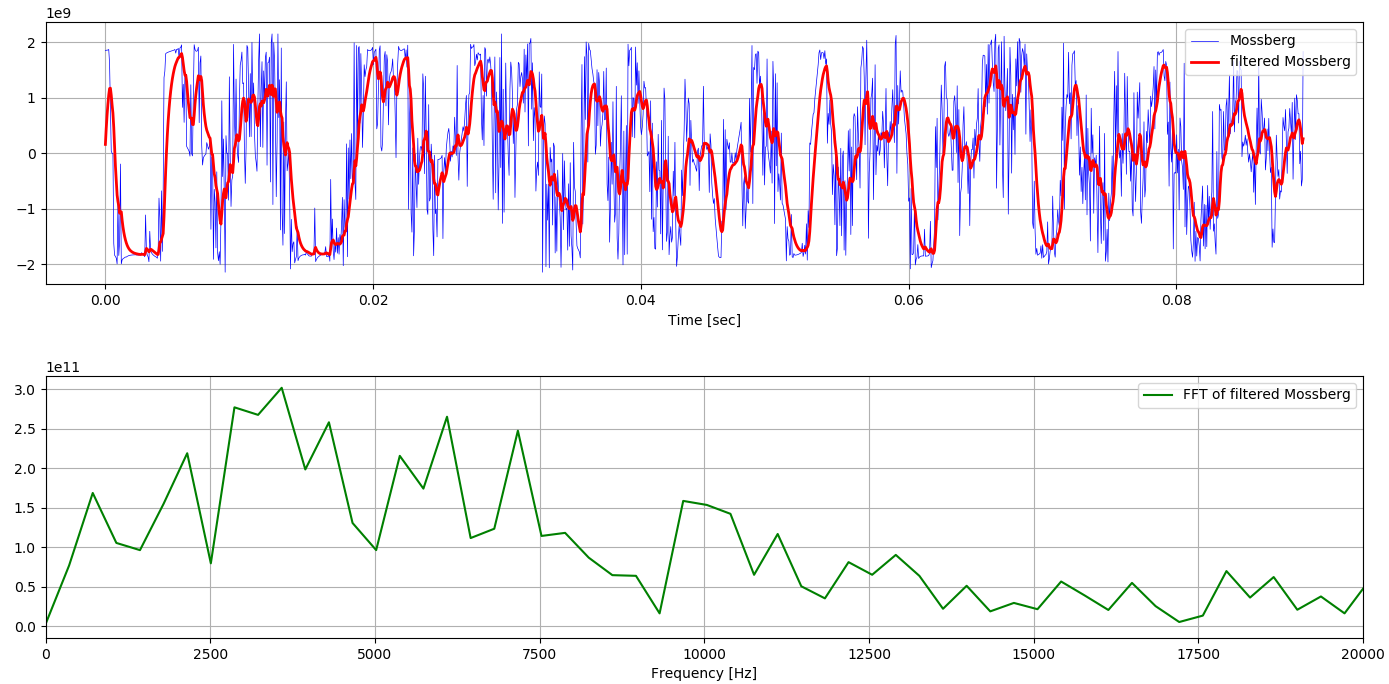
\includegraphics[height=3.9cm]{wykresy/Mossberg_fft.png}
		\subcaption{Mossberg 500}
	\end{subfigure}
	\caption{\label{pic:wykresy_FFt} Wykresy z analiz FFT dźwięków strzałów}
\end{figure}

Mimo, że nie udało się doprowadzić do przedstawienia większej liczby punktów na wykresie FFT, to z pewną dokładnością można stwierdzić, że dla wszystkich dźwięków największy pik mieści się w zakresie $ 3-6kHz $. Dodatkowo na wykresach przedstawiających oryginalny przebieg sygnału widać, że mikrofony w większości przypadków osiągnęły poziom nasycenia (wypłaszczenia na granicach osi y). To wpływa negatywnie na jakość transformaty i oznacza, że dźwięk osiągnął poziom nasycenia mikrofonu, która zwykle wynosi między $ 110 $ a $ 130 dB $. 

Powyższa analiza wskazuje na to, że zarówno częstotliwości, jak i natężenia dźwięków strzałów z broni palnej czyni je szczególnie niebezpiecznymi dla słuchu.

	
	\chapter{Zalozenia projektowe}
\label{cha: zalozeniaprojektowe}

Głównym założeniem tej pracy inżynierskiej było wykonanie strzeleckich ochronników słuchu. Zamysł był wzorowany na istniejących produktach, choć miał rozszerzać ich funkcjonalność. Słuchawki miały składać się z materiału tłumiącego, elektronicznego układu przetwarzania dźwięku z otoczenia oraz złącza do komunikacji radiowej. Elektroniczny układ spełniał główne zadanie w słuchawkach, ponieważ przekazywał dźwięk z otoczenia oraz z radiotelefonu do ucha użytkownika, aby materiał tłumiący nie zakłócał normalnej komunikacji oraz dokonywał aktywnego wyciszenia dźwięków, podobnie jak w słuchawkach multimedialnych, kiedy natężenie fali akustycznych przekraczało określony poziom.

Słuchawki miały być stworzone od podstaw aż do otrzymania gotowego produktu, co obejmowało:

\begin{itemize}
	\item dobór parametrów głośników, mikrofonów, baterii i innych elementów
	\item zaprojektowanie, zamówienie i zlutowanie płytki PCB
	\item napisanie oprogramowania do mikrokontrolera przetwarzającego sygnały
	\item zaprojektowanie i wydrukowanie na drukarce 3D obudowy słuchawek
	\item dobór materiału tłumiącego pasywnie
\end{itemize}

\chapter{Istniejące rozwiązania}

\textbf{JAK DZIAŁAJĄ TAKIE SORDINY}
	\chapter{Hardware}
\label{cha:hardware}

Największą częścią projektu było wykonanie hardware'u słuchawek. Dobór parametrów elementów akustycznych był szczególnie trudny, biorąc pod uwagę brak doświadczenia w tym obszarze elektroniki. Wszystkie elementy schematu musiały być wybrane pod kątem minimalizacji szumów i poboru mocy, a zaprojektowana płytka musiała się zmieścić do obudowy słuchawek i pozwolić na wyprowadzenie na zewnątrz mikrofonu, przycisków oraz gniazda ładowania. To wymagało przemyślanego wymiarowania zarówno modelu, jak i płytki oraz wyprowadzenia w odpowiedni sposób elementów, na przykład stosując kątowe przyciski.

Dla projektu obudowy głównym ograniczeniem było to, aby słuchawki były kompaktowe, czyli lekkie i niskoprofilowe. Ochronniki tego typu są przeznaczone dla myśliwych, strzelców sportowych, ale również dla służb ochrony i wojsk specjalnych. Toteż nie mogą ograniczać ruchów, możliwości przyłożenia głowy do kolby broni i być znaczącym ciężarem podczas użytkowania przez kilka godzin lub dni w terenie.

Ten sam powód determinuje wymóg niskiego poboru prądu przez układ i dużej pojemności akumulatora. Choć w tej pracy został wybrany wbudowany akumulator ładowany przez gniazdo mikro USB, to do zastosowań wojskowych lepsze byłoby zasilanie ze zwykłych, wymiennych baterii, na przykład AAA.

Układy scalone zastosowane w projekcie musiały mieć możliwość zasilania napięciem 3.3V, ponieważ zastosowany został akumulator litowo-jonowy o napięciu znamionowym $3,7V$ (zakres pracy wynosi od $3,0$ do $4,2V$).

Dla uproszczenia, podczas wyboru komponentów nie była brana pod uwagę wodo- oraz kurzoodporność i zakres temperatur pracy. Jednak gdyby słuchawki miały wejść na rynek, musiałyby zostać dodatkowo przystosowane do działania w wymagających warunkach terenowych.


\section{Układ elektroniczny}
\label{cha:uklad}

Przed przystąpieniem do projektowania właściwego układu elektronicznego konieczne było zadecydowanie, czy wykonać go analogowo, czy cyfrowo. Podejście pierwsze oznaczało użycie inwerterów, wzmacniaczy, filtrów, itp. do uzyskania odpowiednich opóźnienia i fazy dźwięku. Jednak pozostawała wciąż kwestia możliwości zamiennego wyciszania i przekazywania dźwięków w zależności od ich amplitudy. Okazało się, że znalezienie materiałów na ten temat jest wyjątkowo trudne, a szukanie błędów na schemacie mogłoby sprawiać dużo więcej problemów, niż w programie na mikrokontroler. Z tego powodu został wybrany układ cyfrowy, który jak się później okazało, powodował wiele problemów z szumami i opóźnieniami sygnału.

Kolejną decyzją do podjęcia było to, czy każda ze słuchawek będzie miała swój własny układ, czy też jedna będzie odpowiedzialna za obliczenia, a druga jedynie skomunikowana z nią. Zostało wybrane podejście drugie, ponieważ pozwalało to zminimalizować koszty oraz lepiej rozłożyć masę. Jedna słuchawka miała zawierać główną płytkę z mikrokontrolerem i przyciskami, a druga jedynie mikrofon oraz układ ładowania i akumulator. Wadą tego rozwiązania była konieczność równoczesnej analizy dźwięków z obu słuchawek, co przekładało się na szybkość działania mikrokontrolera oraz narażone na szumy przewody prowadzące przez pałąk od jednej słuchawki do drugiej.

Poniżej przedstawiono uproszczony schemat układów dla obu słuchawek.

\textbf{SCHEMAT UKŁADÓW SŁUCHAWEK}


\section{Głośniki}
\label{cha:glosniki}

Każda ze słuchawek została wyposażona w głośnik odpowiedzialny zarówno za doprowadzanie do ucha zwykłych dźwięków z zewnątrz, jak i generowanie antyfazy dla dźwięków niebezpiecznych. Wybrany został głośnik \textit{254-PS604-RO} firmy \textit{Kobitone}. Głównym kryterium wyboru była impedancja głośnika, wynosząca $32\Omega$ oraz moc znamionowa na poziomie $ 200 mW $. Te parametry zapewniały dobrą jakość odtwarzanego dźwięku, która była kluczowa, aby uzyskać maksymalne odwzorowanie dźwięków otoczenia. Celem było to, aby użytkownik czuł się w słuchawkach naturalnie. Choć charakterystyka częstotliwościowa głośnika jest zbliżona do liniowej tylko w zakresie od $ 400 $ do $ 7000 Hz $, to zawiera się w nim większość słyszanych odbieranych przez człowieka dźwięków.

Sterowanie głośnikami zostało przewidziane z wykorzystaniem wbudowanych w mikrokontroler dwóch 12-bitowych przetworników cyfrowo-analogowych w trybie single-ended. Ich wyjścia były dodatkowo wzmacniane przez układy \textit{TPA2005D1DGNR} firmy \textit{Texas Instruments}. Są to wzmacniacze audio klasy D, stworzonej na potrzeby urządzeń przenośnych. Obok innych popularnych klas, jak A, B, AB, czy G, klasa D charakteryzuje się bardzo wysoką wydajnością mocową (nawet powyżej $ 90\% $). Wynika ona stąd, że w odróżnieniu od pozostałych, gdzie stosowane są konfiguracje common-emitter lub push-pull, klasa D stosuje całkowite załączanie lub wyłączanie tranzystora wyjściowego i modulację częstotliwości PWM, aby przybliżyć analogowy poziom napięcia\cite{AudioAmps}. Układ \textit{TPA2005D1} ma według specyfikacji wydajność ok. $ 85\% $ przy $32\Omega$ głośniku, zasilaniu $ 3.6V $ i mocy wyjściowej $ 100mW $.

Dodatkowo układy te mają wbudowany pin shutdown, który został użyty aby wyłączać je w trybie uśpienia słuchawek opisanym szerzej w rozdziale \textbf{REF DO ROZDZIALU Z SYSTEMEM SŁUCHAWEK}. Dzięki niemu wzmacniacze mogą pobierać zaledwie $ 0.5 µA $.

W idealnym przypadku słuchawki powinny zawierać kilka głośników, co umożliwiłoby symulację dźwięku przestrzennego. To jednak zwiększyłoby koszt słuchawek, wymagało zamontowania kilku mikrofonów, utrudniło rozmieszczenie elementów wewnątrz i implementację algorytmu wyciszającego.


\section{Mikrofony}
\label{cha:mikrofony}

Wybór mikrofonu był największym problemem ze względu na różne technologie wykonania (elektretowy, MEMS) oraz dużo różnych parametrów. Początkowo miał to być mikrofon elektretowy, jednak okazało się, że są one mało precyzyjne. Konieczne było wybranie technologii MEMS, czyli miniaturowego mikrofonu wbudowanego w chip z otworem do akwizycji fal akustycznych.

\begin{figure}[H]
	\centering
	\begin{subfigure}{.45\textwidth}
		\centering
		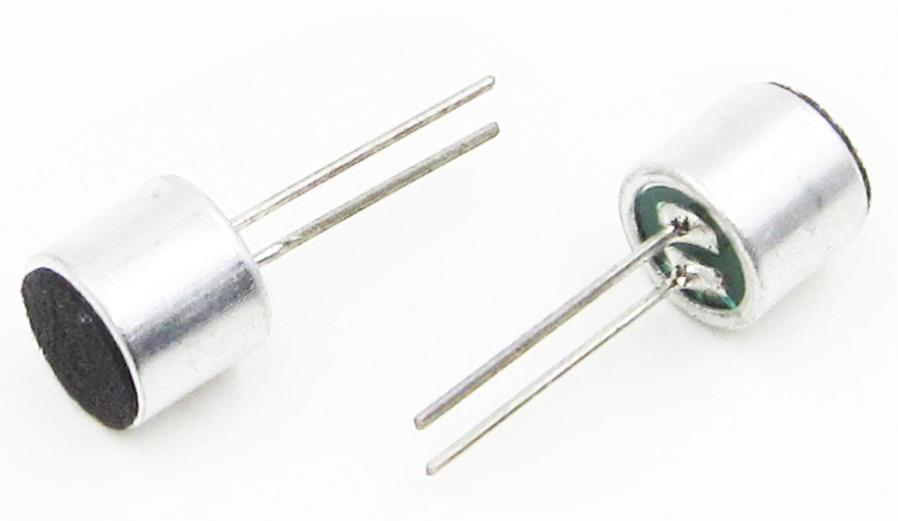
\includegraphics[height=3.5cm]{zdjecia/mic_electret.jpg}
		\subcaption{Mikrofon eletretowy}
	\end{subfigure}
	\begin{subfigure}{.45\textwidth}
		\centering
		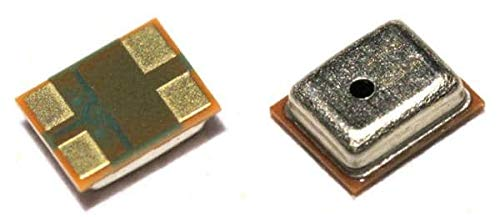
\includegraphics[height=3.5cm]{zdjecia/mic_mems.jpg}
		\subcaption{Mikrofon MEMS}
	\end{subfigure}
	\caption{\label{mikrofony} Mikrofony w różnych technologiach}
\end{figure}

Do celów projektu wybrany został mikrofon \textit{SPW2430HR5H-B} firmy \textit{Knowles}. Ponieważ jest to urządzenie on-chip, konieczne było dostosowanie projektu tak, aby płytka była maksymalnie blisko zewnętrznej ścianki obudowy. Port do akwizycji znajduje się w górnej części elementu i jest odsunięty o $ 1mm $ od dolnej części, a więc ok. $ 1mm $ od powierzchni PCB.
Jednym z głównych kryteriów wyboru była czułość. Informuje ona, jaka amplituda sygnału wyjściowego mikrofonu odpowiada danemu poziomowi ciśnienia akustycznego. W specyfikacji podawana jest jako ujemna wartość $dBV/Pa$ mierzona falą akustyczną o częstotliwości $1kHz$ i SPL $94dB$. Jednostka $dBV$ oznacza liczbę decybeli w odniesieniu do $1V$\cite{MicSens}. Stąd wzór na czułość wygląda następująco:

\begin{equation}
Sensitivity_{dBV} = 20 \cdot log_{10}\frac{Sensitivity_{mV/Pa}}{Output_{REF}}
\end{equation}

gdzie: \\
\indent$Sensitivity_{dBV}$ - czułość w dBV/Pa \\
\indent$Sensitivity_{mV/Pa}$ - czułość w mV/Pa \\
\indent$Output_{REF}$ - wyjściowe napięcie odniesienia ($1000mV/Pa$) 

Powyższy wzór można przekształcić, aby z podanej w nocie katalogowej czułości obliczyć poziom napięcia dla danego SPL.
\begin{equation}
Sensitivity_{mV/Pa} = 1000 \cdot 10^{\frac{Sensitivity_{dBV}}{20}}
\end{equation}

Wybrany mikrofon ma średnią czułość $-42 dbV/Pa$, a więc zgodnie ze wzorem $7,943 mV/Pa$. Stąd przy poziomie ciśnienia akustycznego $1Pa$ zmiana sygnału wyjściowego mikrofonu wyniesie $7,943 mV$. Według specyfikacji maksymalny poziom SPL to $129 dB$, czyli $56,37 Pa$. Maksymalną zmianą napięcia wyjściowego mikrofonu powinno być więc $447,75 mV$.

Czułość mikrofonu jest zwykle odwrotnie proporcjonalna do jego maksymalnego SPL. Dlatego w projekcie słuchawek strzeleckich, które są przeznaczone do nasłuchiwania zarówno skrajnie cichych, jak i skrajnie głośnych dźwięków, zastosowanie jednego mikrofonu wymaga kompromisu między oboma parametrami. 

Rozwiązaniami w tej sytuacji byłoby zastosowanie dwóch mikrofonów o różnych czułościach lub dodanie wzmacniacza sterowanego przez oprogramowanie. Pierwsze z nich gwarantuje dobrą akwizycję wszystkich poziomów dźwięków, jednak jest wyzwaniem pod względem konstrukcyjnym, wymaga użycia większej liczby przetworników analogowo-cyfrowych i sprawnego przełączania przetwarzania przez oprogramowanie. Drugie zaś bazowałoby na mikrofonie o małej czułości i przy małych natężeniach dźwięku zwiększaniu jego amplitudy wyjściowej przez wzmacniacz sterowany potencjometrem cyfrowym. To rozwiązanie wydaje się być lepsze, choć również wymaga zaprogramowania portów mikrokontrolera tak, aby dostosowywały wzmocnienie.

W tym konkretnym przypadku problemem jest konieczność przetwarzania dźwięków o amplitudach przekraczających $140dB$
\textbf{REFERENCJA}
Znalezienie mikrofonu z takim wysokim progiem jest bardzo trudne, dlatego prawdopodobnie konieczne by było mechaniczne wyciszenie dźwięków docierających do mikrofonu, aby obniżyć odbierany poziom ciśnienia akustycznego.

Słuchawki zostały dodatkowo zaprojektowane tak, aby była możliwość podłączenia ich do radiotelefonu. Do tego celu został wybrany jeszcze jeden mikrofon montowany w elastycznej rurce przed ustami użytkownika i umożliwiający rozmowę z użyciem komunikacji radiowej. W tym przypadku jest to mikrofon elektretowy \textit{CMEJ-4622-25-L082}, ponieważ jego montaż nie wymaga padów lutowniczych. Nie było konieczne wybieranie mikrofonu o dobrym SNR, ponieważ komunikacja radiowa i tak wprowadza duże szumy. Czułość mikrofonu powinna być natomiast stosunkowo mała, ponieważ odległość od źródła dźwięku jest niewielka.


\section{Mikrokontroler}
\label{cha:uC}

Jako jednostkę obliczeniową, wybrano mikrokontroler firmy \textit{STMicroelectronics}: \textit{STM32L476RG}.

Jego rdzeniem jest 32-bitowy \textit{Cortex-M4} z możliwością zastosowania bibliotek DSP (ang. \textit{Digital Signal Processing} - Cyfrowe Przetwarzanie Sygnałów). Z kolei \textit{L} jest niskoprądową alternatywą dla serii \textit{F}. Głównie tych dwóch powodów został wybrany do tych słuchawek.

Maksymalna częstotliwość zegara procesora wynosi $80MHz$. Mikrokontroler posiada 3 12-bitowe przetworniki analogowo-cyfrowe, czyli akurat tyle, aby próbkować dwa mikrofony i sygnał z radiotelefonu. Do tego 2 12-bitowe przetworniki cyfrowo-analogowe - po jednym na głośnik\cite{STM32L4}.

Na potrzeby prototypowania wykorzystano płytkę \textit{Nucleo-64}, która zawiera programator \textit{ST-LINK}, diodę oraz przycisk użytkownika, przycisk resetu i jest kompatybilna z nakładkami na popularną platformę \textit{Arduino Uno}. Miała ona zostać również użyta do zaprogramowania mikrokontrolera na docelowej płytce PCB.


\section{PCB}
\label{cha:PCB}

Projekt płytki PCB został wykonany w programie \textit{Altium Designer 6.1} na licencji AGH udostępnionej przez Promotora. Postępy były archiwizowane z użyciem systemu kontroli wersji \textit{git}. Repozytorium z projektem: \url{https://gitlab.com/Hoplophile/tactical_headphones.git}.

Zastosowano globalne etykiety połączeń i podział na pliki dla lepszej przejrzystości. Do wyglądu schematów wykorzystany został szablon stworzony w ramach zajęć \textit{Podstawy projektowania obwodów z wykorzystaniem oprogramowania CAD/CAM}. 

Ponieważ użyta wersja \textit{Altiuma} nie posiada jeszcze opcji projektu wielolayoutowego, konieczne było stworzenie dwóch podprojektów. Zostały do nich dodane odpowiednie pliki z głównego projektu. Strukturę plików przedstawiono na obrazku \ref{pic:struktura}.

\begin{figure}[H]
	\centering
	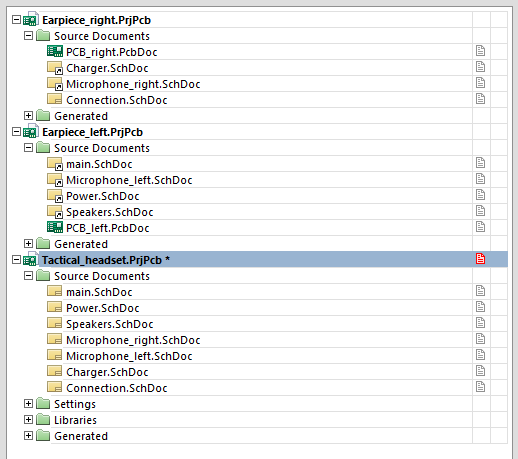
\includegraphics[scale=0.6]{zdjecia/PCB/struktura.png}
	\caption{\label{pic:struktura} Struktura plików w projektach PCB}
\end{figure}

Poniżej opisano poszczególne schematy oraz layouty składające się na projekt słuchawek.


\subsection{Main}

Plik main.sch zawiera ogólne elementy schematu, czyli: mikrokontroler, przyciski użytkownika oraz konektory do programowania, komunikacji między lewą i prawą słuchawką, mikrofonu komunikacyjnego i komunikacji radiowej.

Przewidziano 3 przyciski dla użytkownika (plus/góra, minus/dół, główny). Zostały podłączone do portów GPIO mikrokontrolera oraz do zasilania przez rezystory pull-up o wartościach $4,7k\Omega$. Wciśnięcie przycisku jest równoważne ze zwarciem danego portu do masy.

Podobnie pin \textbf{NRST} jest podłączony do zasilania przez rezystor pull-up. W pierwszych wersjach schematu był tam również podłączony przycisk TACT, jednak usunięto go, aby zaoszczędzić miejsce. Reset jest możliwy poprzez zwarcie pinu resetu na konektorze \textbf{SWD}.

Złącze do programowania jest zaprojektowane tak, aby można było flashować i debugować mikrokontroler przez złącze ST-LINK obecne na przykład na platformie Nucleo, na której wykonywany był prototyp. 

Konektor do komunikacji radiowej ma 3 piny. Pierwszy jest połączeniem do masy. Drugi przekazuje sygnał z radiotelefonu do przetwornika analogowo-cyfrowego mikrokontrolera. Trzeci jest pinem wyjściowym mikrofonu komunikacyjnego, przy którym zastosowano równolegle rezystor, ograniczający prąd zasilania mikrofonu oraz szeregowo kondensator blokujący napięcie stałe.

Do pinu $V_{REF}$ mikrokontrolera dodano dodatkowo dwa kondensatory: \textbf{C1} i \textbf{C4}. Zastosowano je później, po pierwszych próbach odczytu sygnału z mikrofonu przez wbudowany ADC, ponieważ okazało się, że jest on obarczony dużym szumem.

\begin{figure}[H]
	\centering
	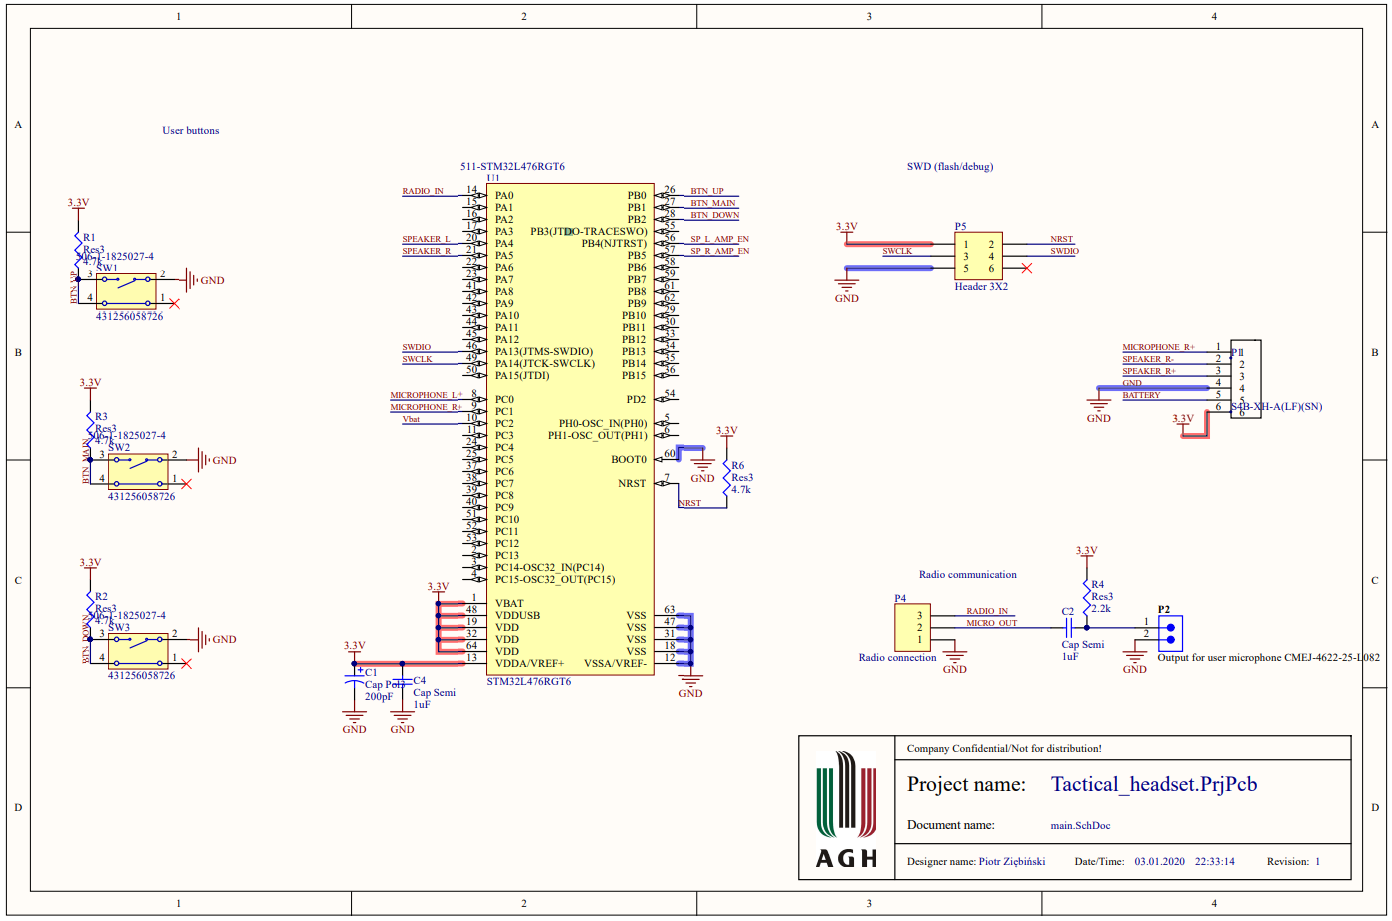
\includegraphics[scale=0.4]{zdjecia/PCB/main.png}
	\caption{\label{main} Schemat \textit{main}}
\end{figure}


\subsection{Power}

Początkowo ten plik zawierał stabilizator napięcia oraz układ ładowania do akumulatora. Na potrzeby podziału układu na dwie osobne płytki PCB, układ ładowania został przeniesiony na osobny schemat. Na głównej, lewej płytce został stabilizator \textbf{JAKI STABILIZATOR} ustawiony na $3.3V$. Według specyfikacji jest w stanie dać \textbf{PRĄD}. Zostały dodane kondensatory filtrujące oraz cewka na wyjściu, tworzące filtr dolnoprzepustowy LC o częstotliwości granicznej \textbf{CZESTOT. NA WYJŚCIU REG}. 

Miedzy portem wejściowym baterii a masą został utworzony dzielnik napięcia z rezystorami $220k \Omega $. Było to konieczne do pomiaru poziomu naładowania baterii, ponieważ jej napięcie maksymalne wynosi $4,2V$ co wykracza poza zakres przetwornika mikrokontrolera, którego $V_{ref}$ wynosi $3,3V$. Napięcie jest dzielone przez 2, więc maksymalnie wynosi $2,1V$ i mieści się w zakresie ADC, a odczytana wartość jest mnożona dwukrotnie przez program, aby otrzymać rzeczywistą wartość. Dzięki zastosowaniu rezystorów o dużej wartości, prąd przepływający przez dzielnik przy pełnym naładowaniu baterii wynosi tylko $9,6\mu A$.

\begin{figure}[H]
	\centering
	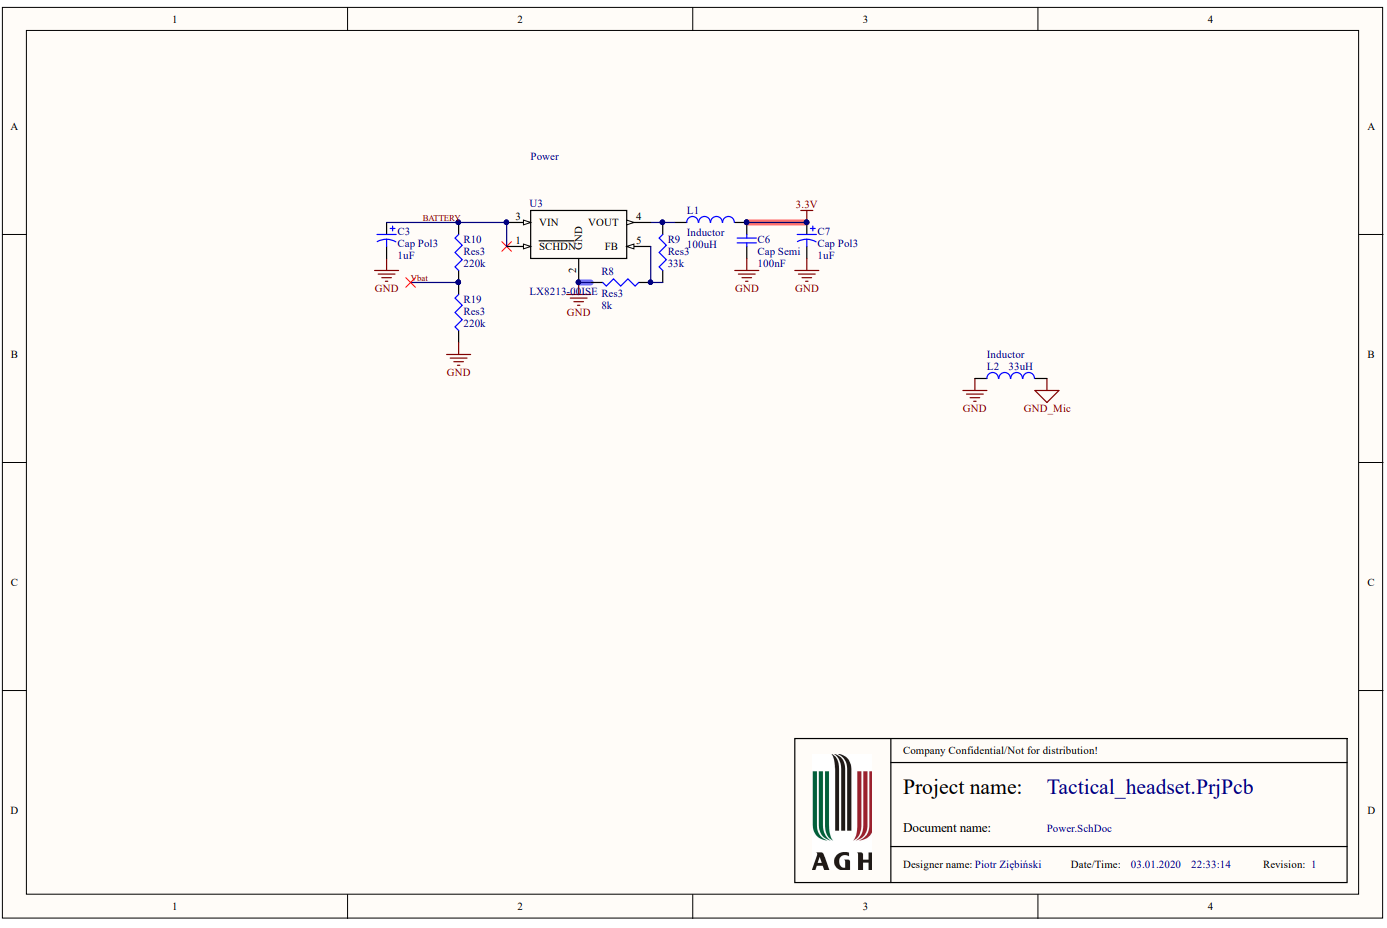
\includegraphics[scale=0.4]{zdjecia/PCB/power.png}
	\caption{\label{power} Schemat \textit{Power}}
\end{figure}


\subsection{Charger}

Układ ładujący do akumulatora został przeniesiony na osobny schemat, kiedy zdecydowano o jego umieszczeniu na drugiej płytce. Wejściem jest złącze żeńskie micro USB B, przez które dostarczane jest napięcie $5V$, natomiast wyjście jest bezpośrednio połączone z portem akumulatora. Wykorzystano również możliwość wskazywania statusu ładowania, dodając diodę LED według specyfikacji. Rezystor \textbf{R16} służy do ustawiania prądu ładowania, wybrana wartość jest równoważna z $450mA$, co jest bliskie maksymalnemu prądowi ładowania wybranego akumulatora, wynoszącemu \textbf{PRĄD ŁADOWANIA}. 

Zgodnie z zalecaną aplikacją w nocie katalogowej, dodano kondensatory na wejściu i wyjściu układu.

\begin{figure}[H]
	\centering
	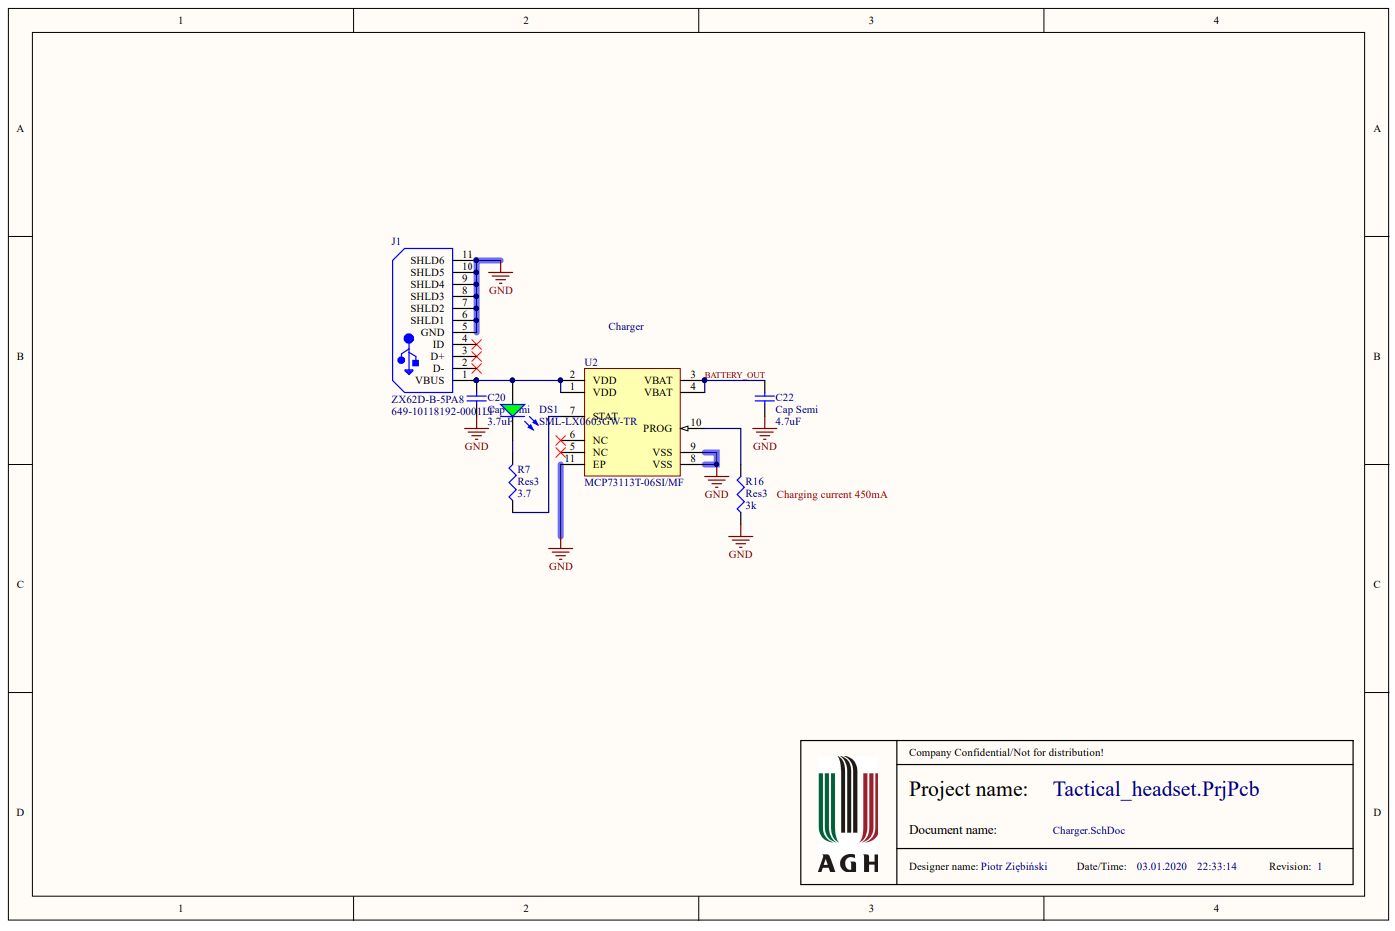
\includegraphics[scale=0.4]{zdjecia/PCB/charger.png}
	\caption{\label{charger} Schemat \textit{Charger}}
\end{figure}


\subsection{Microphone\_left i Microphone\_right}

Oba pliki zawierają bliźniacze schematy z symbolami mikrofonów \textit{SPW2430}. Oprócz nich wstawione zostały kondensatory filtrujące na zasilaniu oraz filtry dolnoprzepustowe RC na wyjściach. Podobnie jak w poprzednim przypadku - pierwotnie jeden schemat został później podzielony na dwa, ponieważ drugi mikrofon znajduje się na drugiej płytce PCB i musi być zamontowany powierzchniowo.

W projekcie zastosowano dwie rozdzielne masy. Na potrzeby filtracji szumów rozważane były różne konfiguracje i ostatecznie zdecydowano o utworzeniu osobnej masy dla mikrofonów, połączonej na obu płytkach indukcyjnością z głównym GND.

\pagebreak
\begin{figure}[H]
	\centering
	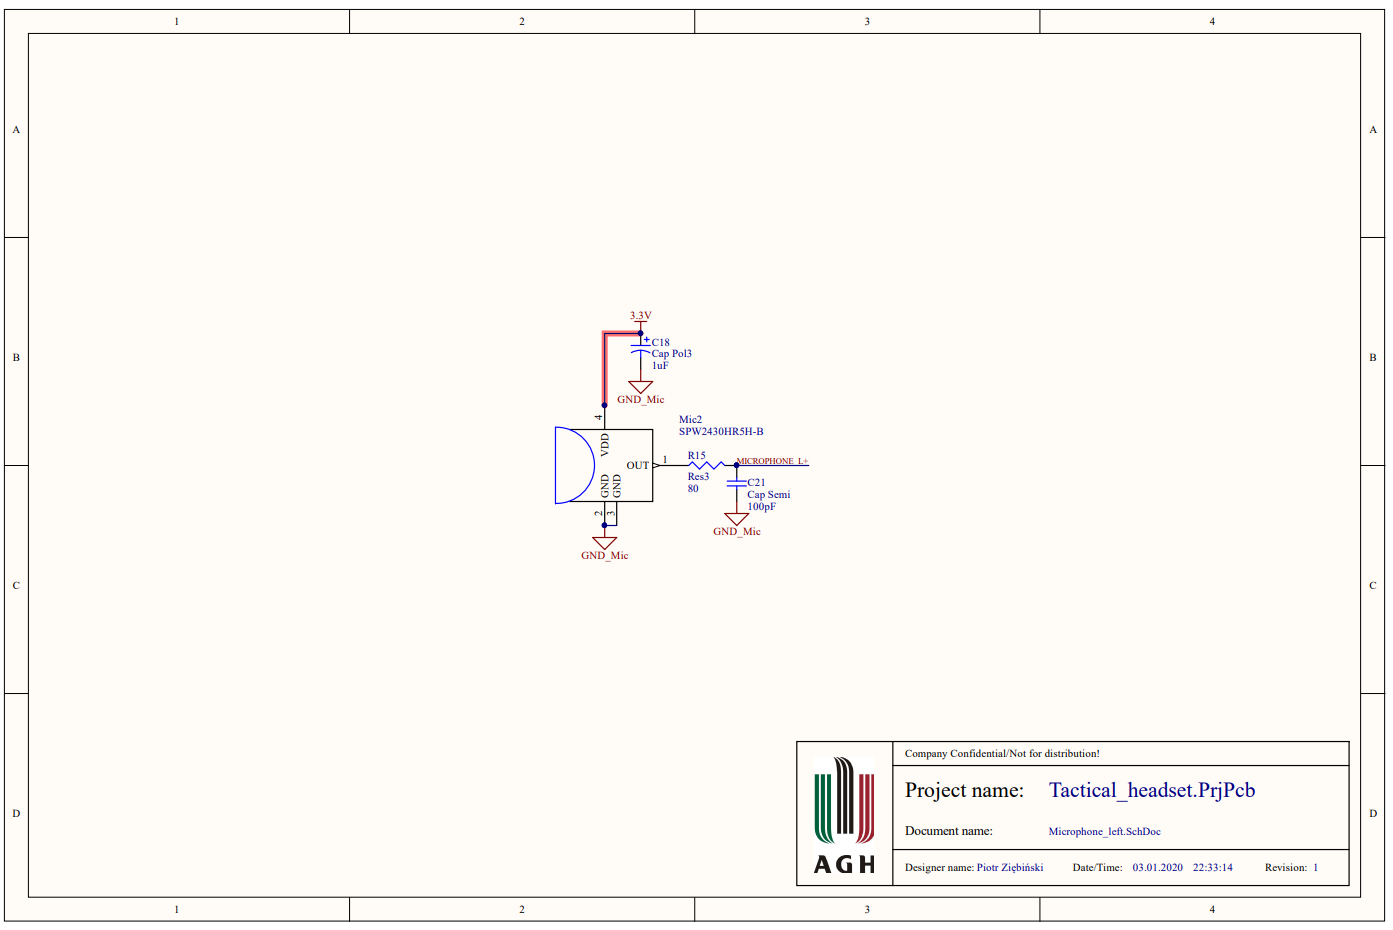
\includegraphics[scale=0.4]{zdjecia/PCB/mic_left.png}
	\caption{\label{mic_left} Schemat \textit{Microphone\_left}}
\end{figure}

\begin{figure}[H]
	\centering
	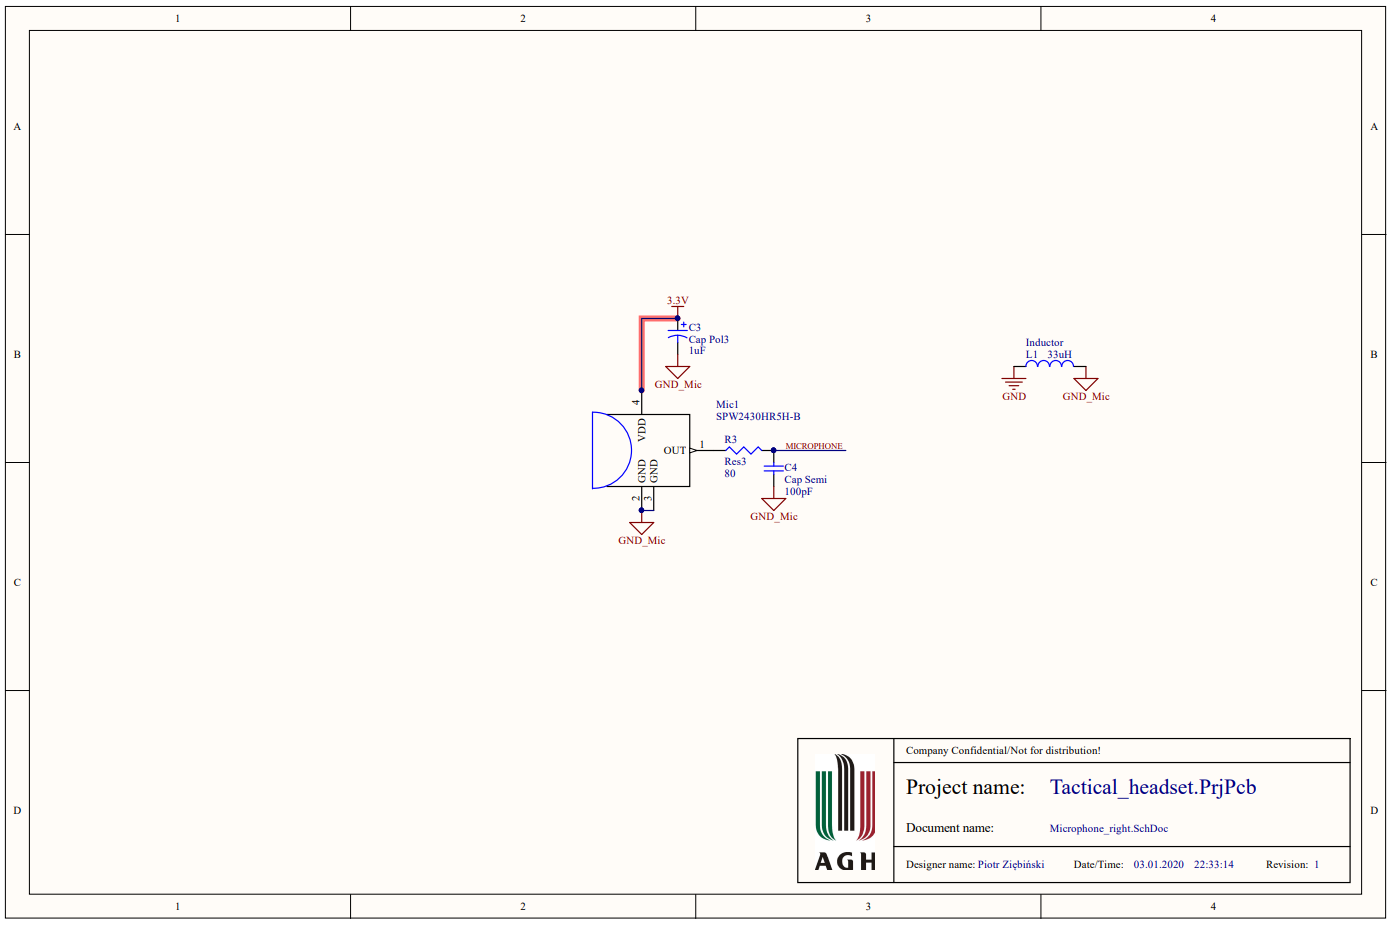
\includegraphics[scale=0.4]{zdjecia/PCB/mic_right.png}
	\caption{\label{mic_right} Schemat \textit{Microphone\_right}}
\end{figure}


\subsection{Speakers}

W przypadku głośników schemat jest wspólny, ponieważ oba wzmacniacze zostały umieszczone na głównym PCB.

Na wyjściach zastosowano filtry LC z częstotliwością graniczną $27khz$ sugerowane w specyfikacji, aby obniżyć szumy EMI. Zasilania również zostały odfiltrowane kondensatorami \textbf{C10} oraz \textbf{C15}.

Na wejściach różnicowych stworzono filtry górnoprzepustowe na $100hz$.

Piny \textbf{SHUTDOWN} zostały podłączone do mikrokontrolera w celu wyłączania wzmacniaczy w trybie uśpienia systemu. Pobierają wtedy maksymalnie $2\mu A$. 

\begin{figure}[H]
	\centering
	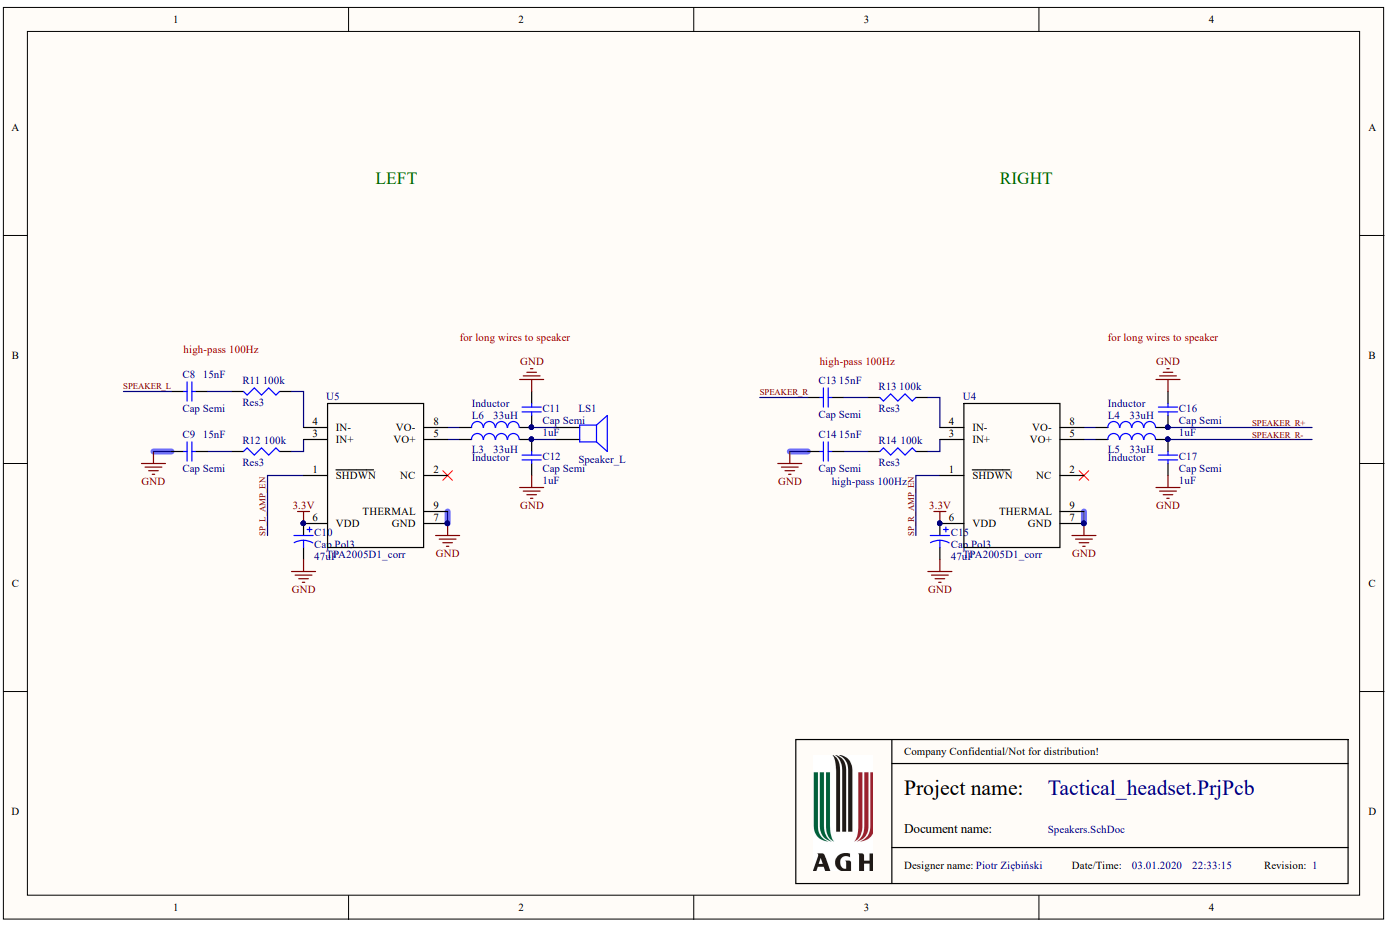
\includegraphics[scale=0.4]{zdjecia/PCB/speakers.png}
	\caption{\label{speakers} Schemat \textit{Speakers}}
\end{figure}


\subsection{Connection}

Schemat stworzony na potrzeby drugiej płytki. Znajdują się na nim: konektor komunikacyjny do głównego PCB, wyjścia do głośnika oraz baterii.

Komunikacja między płytkami odbywa się 6 przewodami: masa, zasilanie $3,3V$, napięcie baterii, dwa sygnały do głośnika i sygnał mikrofonu.

\begin{figure}[H]
	\centering
	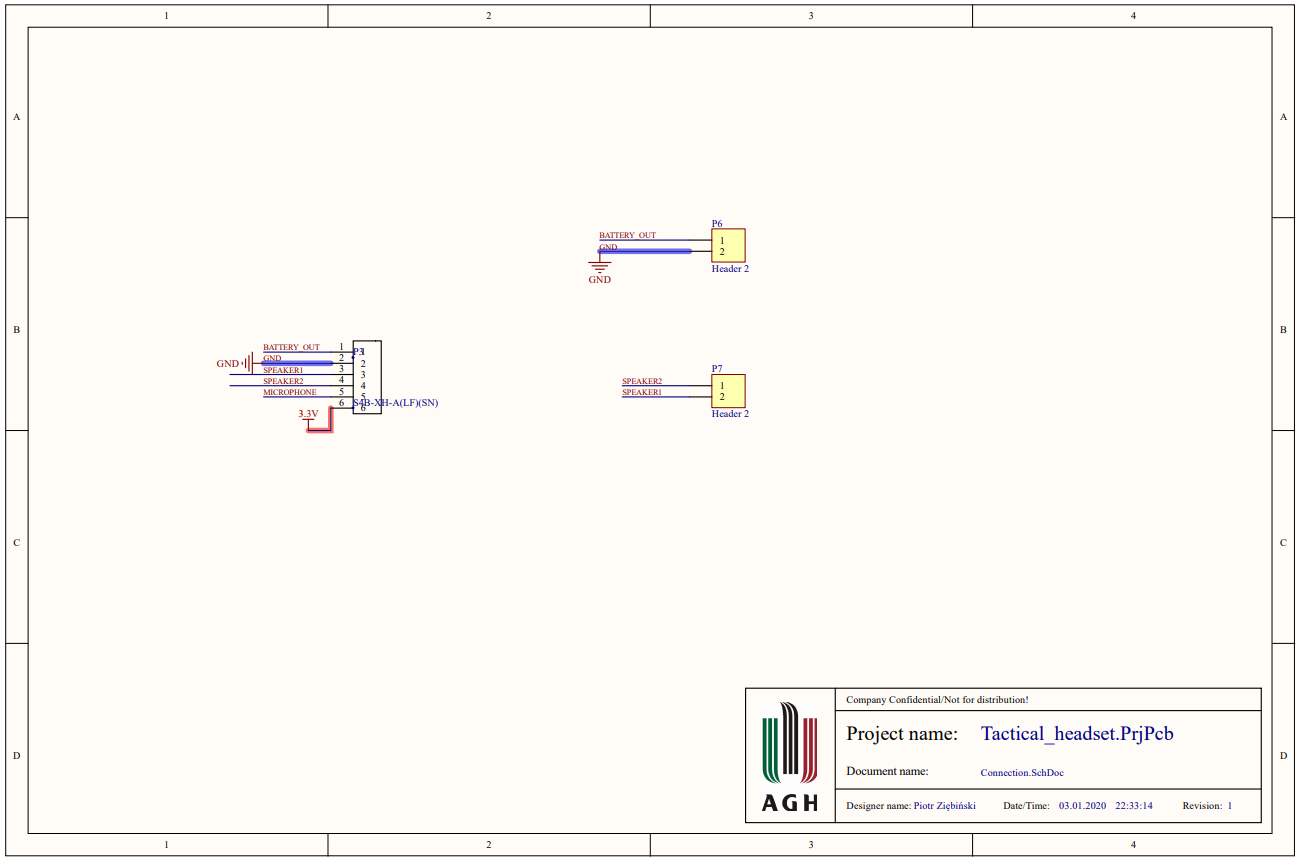
\includegraphics[scale=0.4]{zdjecia/PCB/connection.png}
	\caption{\label{connection} Schemat \textit{Connection}}
\end{figure}


\subsection{PCB\_left}

Jest to główna płytka, na której znajduje się mikrokontroler odpowiedzialny za obliczenia i przetwarzanie sygnałów. Oprócz tego umieszczono na niej przede wszystkim: przyciski, konektor do programowania, do podłączenia radiotelefonu i mikrofonu komunikacyjnego, dwa otwory montażowe wzmacniacze do głośników oraz mikrofon. Ma ona kształt ośmiokąta foremnego o całkowitej szerokości i wysokości $40mm$. Zastosowanie niewielkich wymiarów pozwoliło na łatwe umieszczenie płytki w obudowie i pozostawienie miejsca na materiał wyciszający.

Prawie wszystkie elementy, oprócz mikrofonu i filtrującego jego zasilanie kondensatora, zostały umieszczone na górnej warstwie. Te dwa elementy znajdują się na dole, ponieważ port mikrofonu musiał być skierowany na zewnątrz obudowy i być maksymalnie blisko niej. Do rezystorów zastosowano obudowy 0603, a do kondensatorów i cewek 1206. Utworzone zostały masy \textbf{GND} oraz \textbf{GND\_Mic} na dolnej i górnej warstwie. Związano z nimi także siatkę przelotek łączących obie warstwy ze sobą. Płytka posiada dwa otwory montażowe o średnicach $3,2mm$.

Do mikrofonu komunikacyjnego i połączenia między płytkami zastosowano konektory \textit{JST-XH}. Wyjście głośnika i piny do radiotelefonu przewidziano jako otwory, do których zostaną przylutowane odpowiednie przewody. Natomiast konektor \textbf{SWD} ma służyć jako punkty stykowe do kabla programatora.


\begin{figure}[H]
	\centering
	\begin{subfigure}{.45\textwidth}
		\centering
		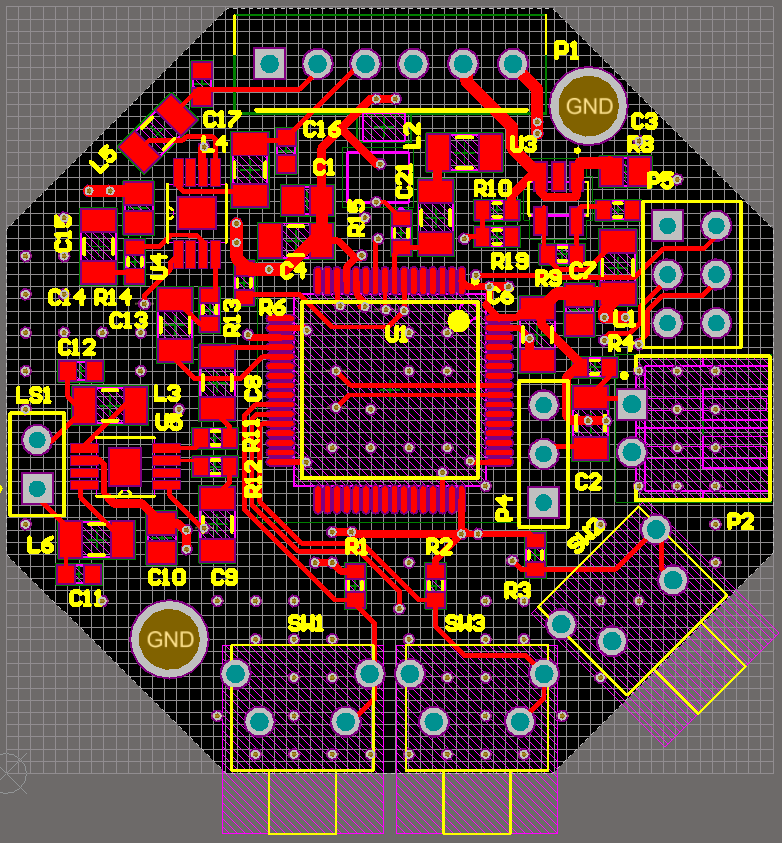
\includegraphics[height=6.5cm]{zdjecia/PCB/PCB_left_top.png}
		\subcaption{Góra}
	\end{subfigure}
	\begin{subfigure}{.45\textwidth}
		\centering
		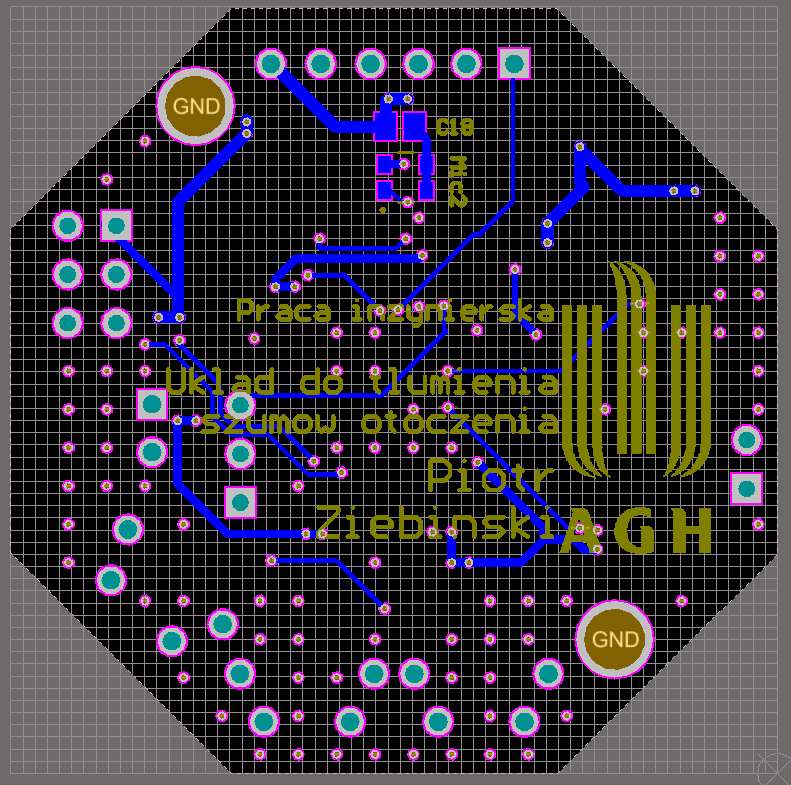
\includegraphics[height=6.5cm]{zdjecia/PCB/PCB_left_bottom.png}
		\subcaption{Dół}
	\end{subfigure}
	\caption{\label{PCB_left} Layout lewej płytki PCB}
\end{figure}

\begin{figure}[H]
	\centering
	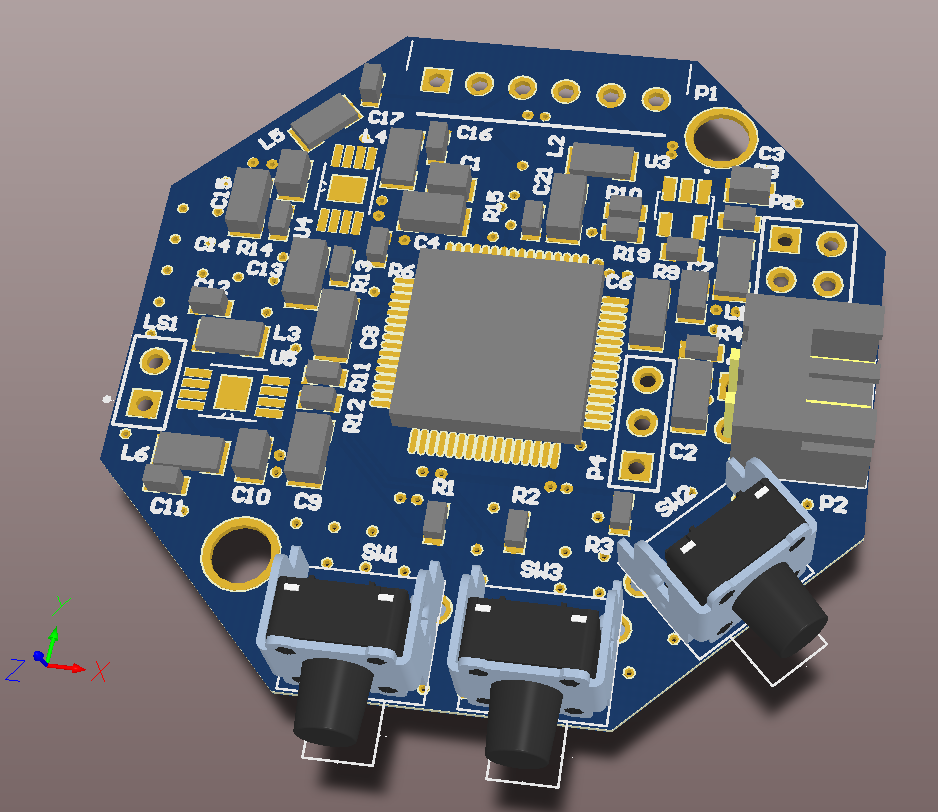
\includegraphics[scale=0.4]{zdjecia/PCB/PCB_left_3D.png}
	\caption{\label{PCB_left_3D} Wygląd płytki z góry w trybie podglądu 3D}
\end{figure}


\subsection{PCB\_right}

Płytka prawa ma znacznie bardziej ograniczoną funkcjonalność. Z tego powodu jej kształt został ograniczony do prostokąta o wymiarach $15x30mm$. 

Podobnie jak w lewej, tylko mikrofon i kondensator na jego zasilaniu, znajdują się na dolnej warstwie. Płytka zawiera oprócz tego konektor do połączenia do drugiej płytki, wyjścia głośnika i baterii oraz układ ładujący z konektorem mikro USB typu B. Również zastosowano tutaj otwory montażowe oraz po dwie masy na warstwę i dla każdej sieć przelotek.

\begin{figure}[H]
	\centering
	\begin{subfigure}{.45\textwidth}
		\centering
		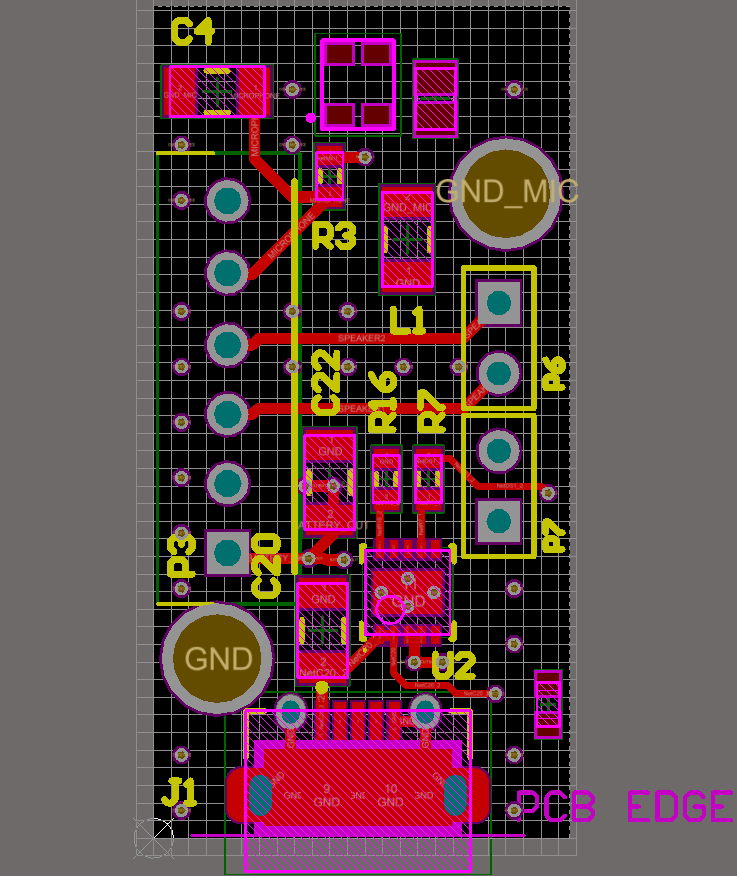
\includegraphics[height=6.5cm]{zdjecia/PCB/PCB_right_top.png}
		\subcaption{Góra}
	\end{subfigure}
	\begin{subfigure}{.45\textwidth}
		\centering
		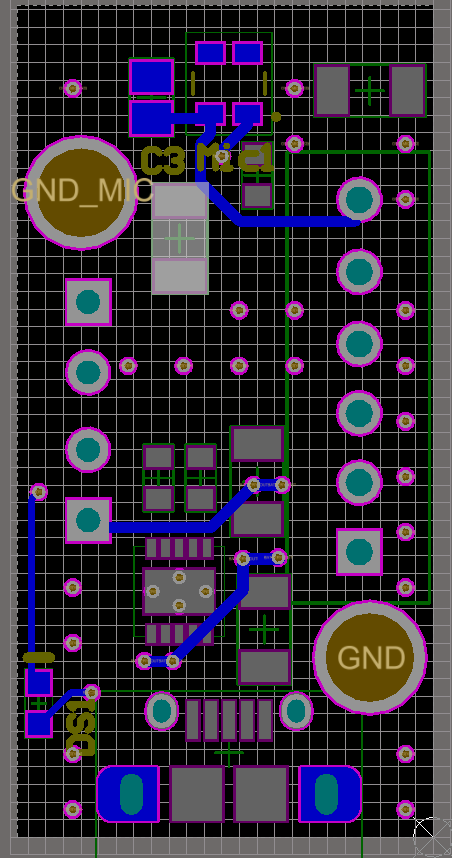
\includegraphics[height=6.5cm]{zdjecia/PCB/PCB_right_bottom.png}
		\subcaption{Dół}
	\end{subfigure}
	\caption{\label{PCB_right} Layout prawej płytki PCB}
\end{figure}

\begin{figure}[H]
	\centering
	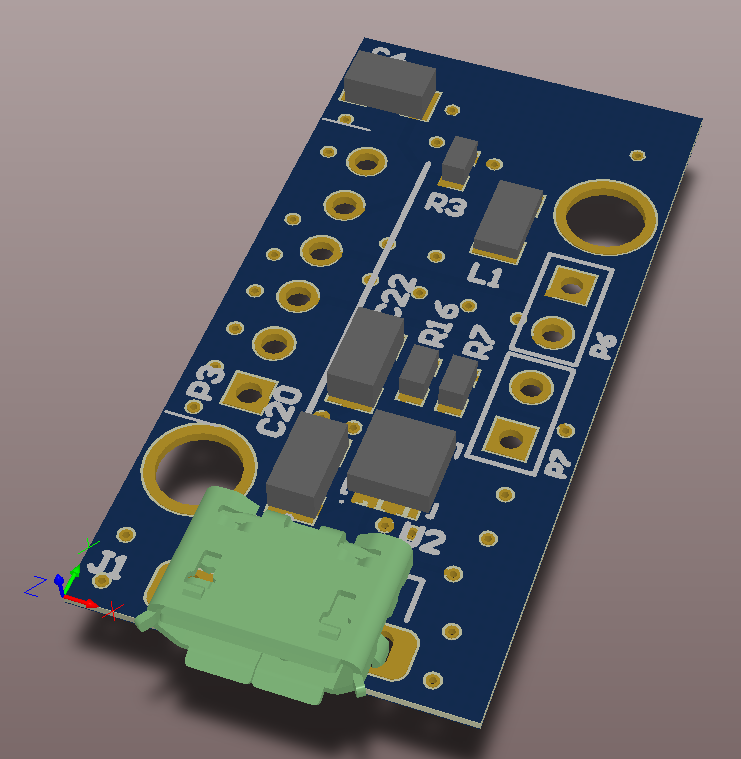
\includegraphics[scale=0.4]{zdjecia/PCB/PCB_right_3D.png}
	\caption{\label{PCB_right_3D} Wygląd prawej płytki z góry w trybie podglądu 3D}
\end{figure}

	
	\chapter{Software}
\label{cha:software}

Oprogramowanie słuchawek zostało napisane w języku C z wykorzystaniem bibliotek HAL, które zawierają dużo gotowych funkcji, na przykład do uruchomienia timera lub do odczytu wartości z przetwornika. Użyto narzędzia \textit{System Workbench for STM32}, które jest zbudowane na popularnym IDE \textit{Eclipse}. Dodatkowo kod do konfiguracji i inicjalizacji peryferiów został wygenerowany z użyciem \textit{CubeMX}.

Tak jak przy pozostałych elementach projektu, wykorzystano repozytorium do zapisywania postępów: \url{https://github.com/Hoplophile/TacticalHeadphones_SW.git}

\begin{figure}[H]
	\centering
	\begin{subfigure}{.48\textwidth}
		\centering
		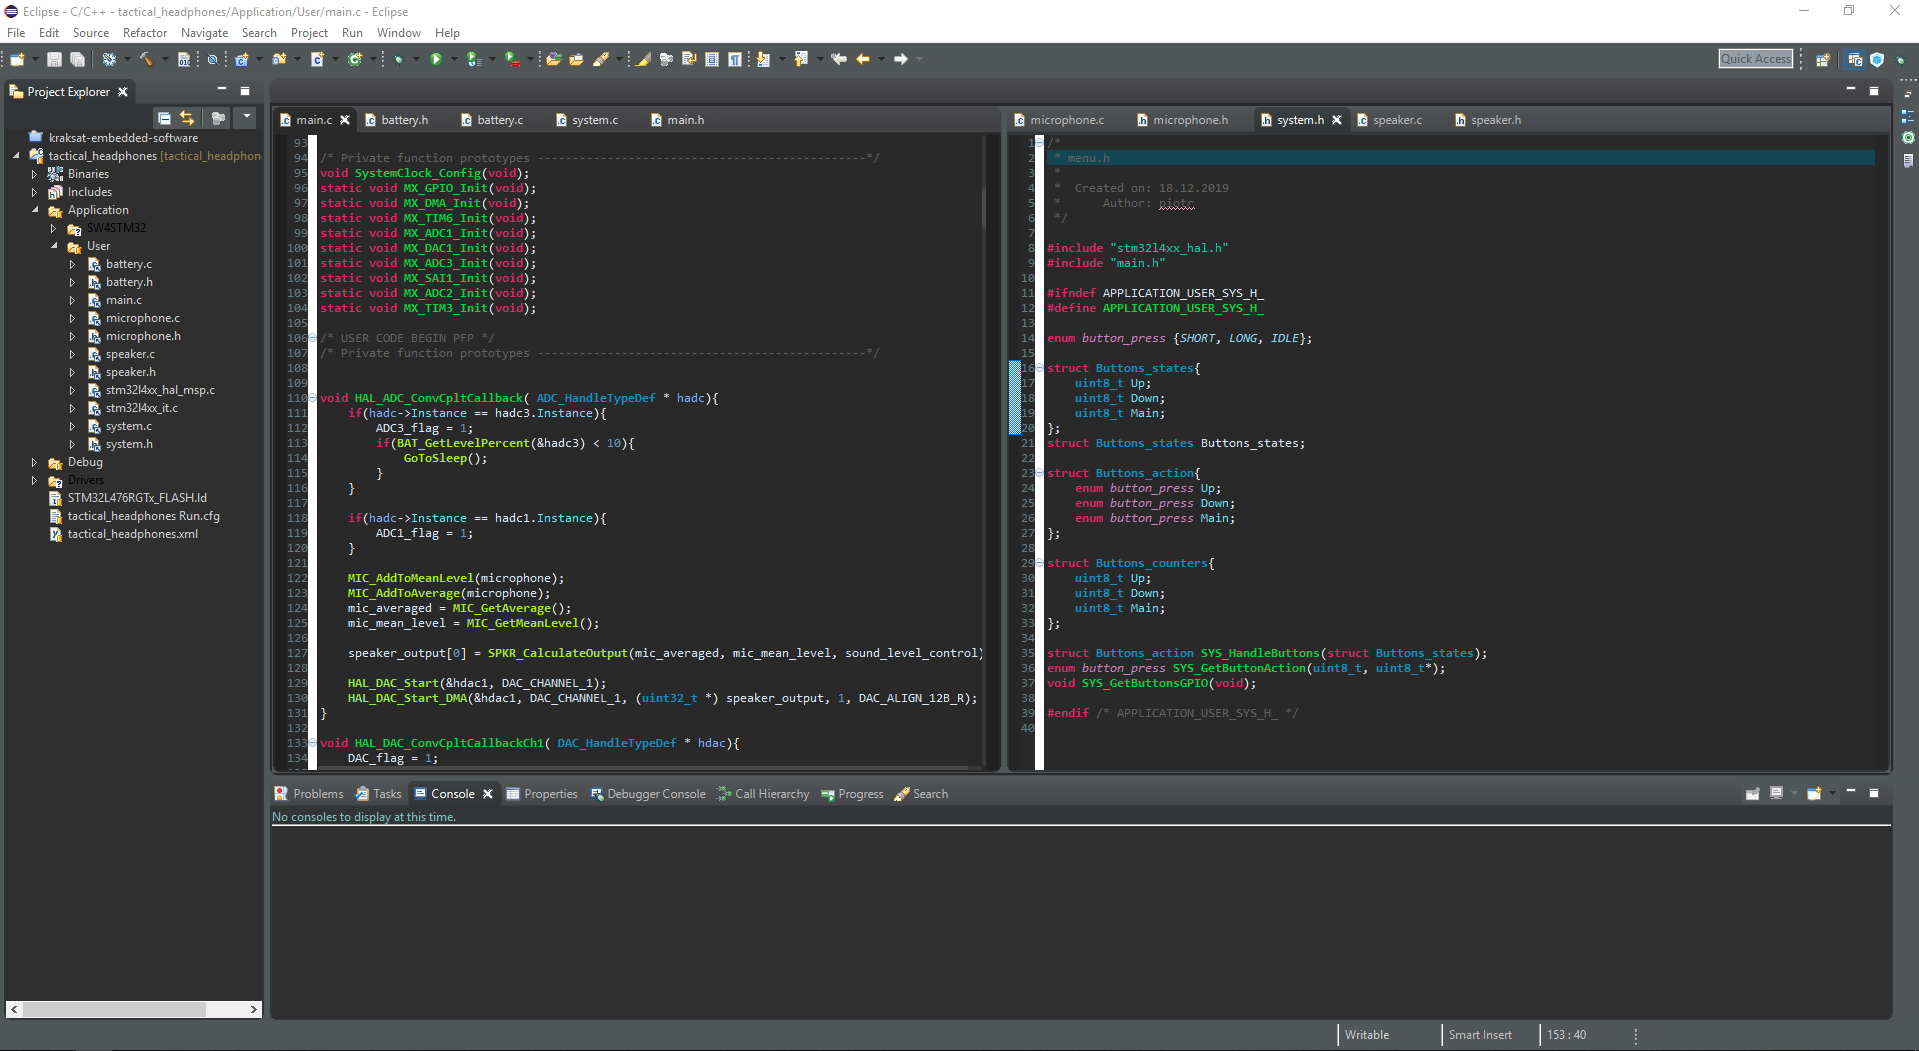
\includegraphics[height=4.2cm]{zdjecia/eclipse.png}
		\subcaption{System Workbench for STM32}
	\end{subfigure}
	\begin{subfigure}{.48\textwidth}
		\centering
		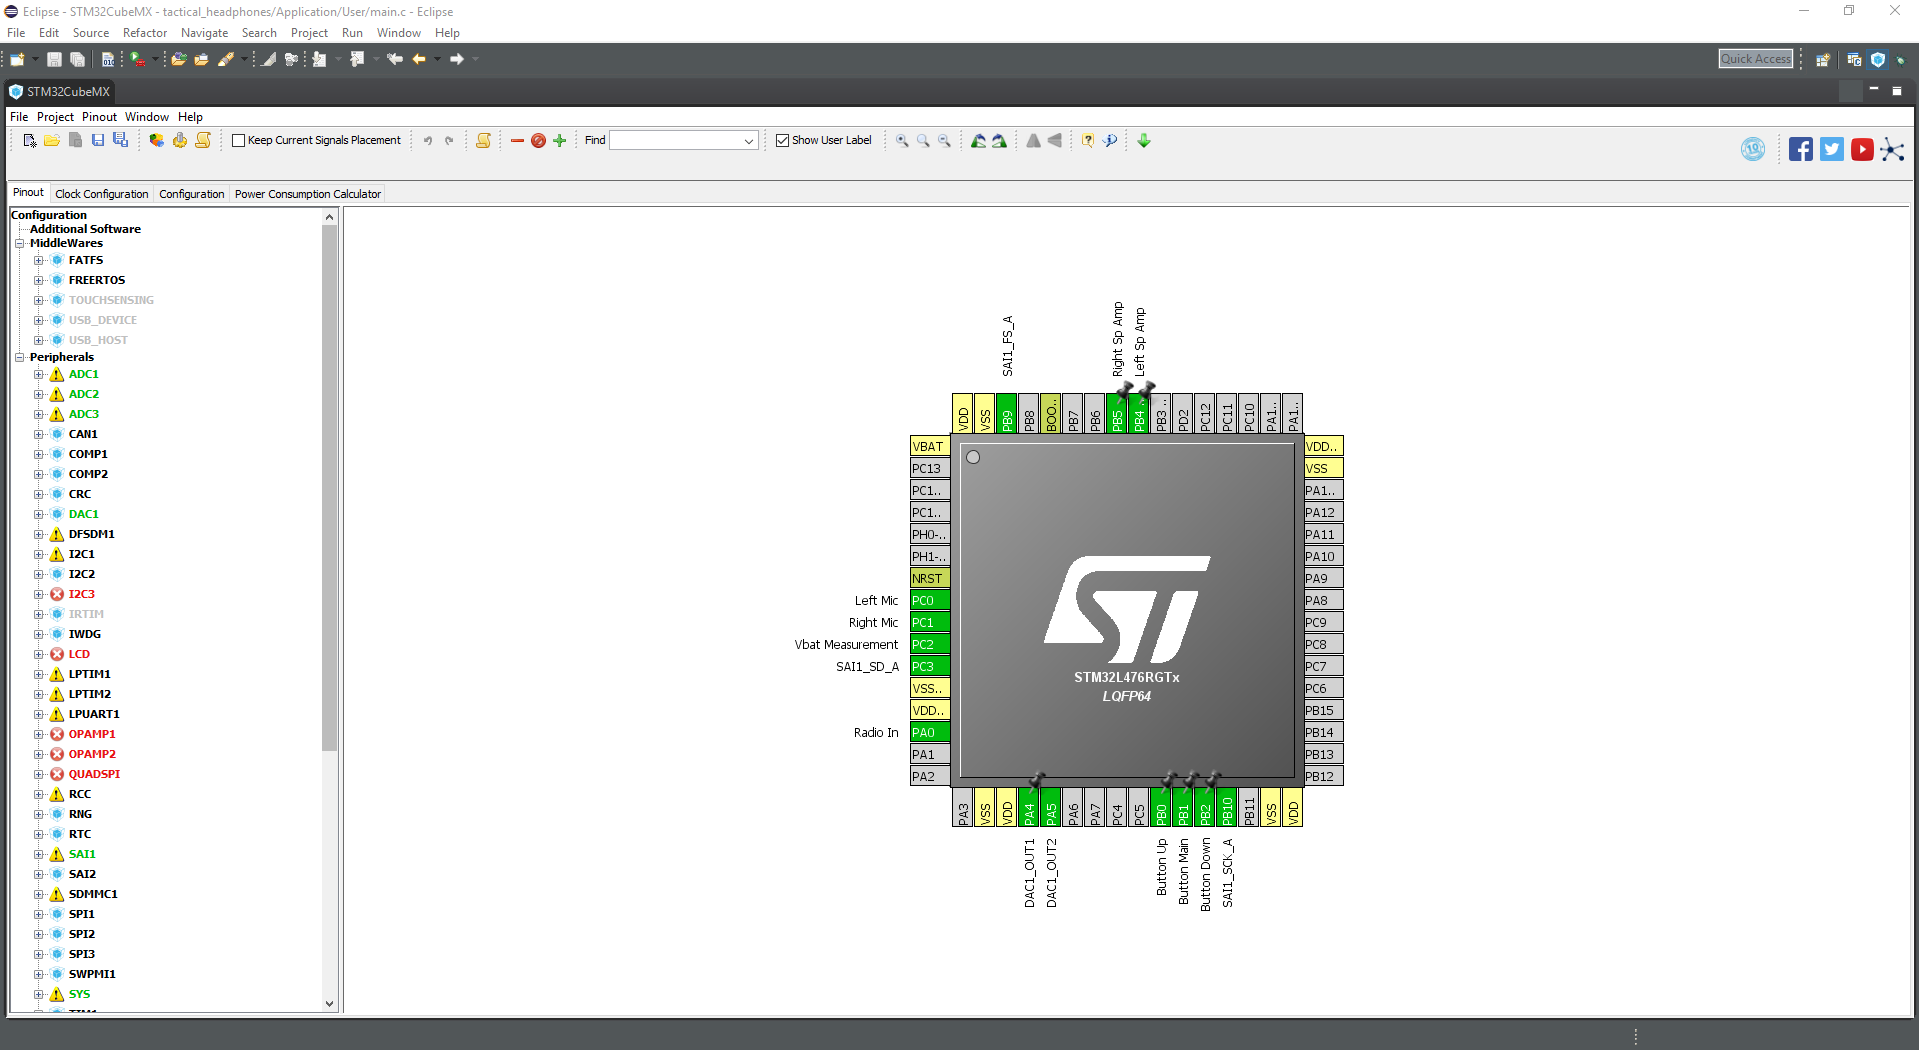
\includegraphics[height=4.2cm]{zdjecia/cubemx.png}
		\subcaption{CubeMX}
	\end{subfigure}
	\caption{\label{pic:IDE} Środowiska użyte do rozwoju oprogramowania}
\end{figure}

Kod był pisany tak, aby rozdzielić program na funkcje wykonujące niewielkie fragmenty. Przewidziano także elastyczną możliwość modyfikacji lub dodawania funkcjonalności, na przykład implementując do $V_{BAT}$ 3 funkcje, odczytujące kolejno: wartość surową, przeliczoną na Volty oraz procenty naładowania. W obecnej wersji użyta została ta ostatnia.

Dla lepszej nawigacji, zastosowano konwencję nazewnictwa funkcji - <NAZWA\_ZWIĄZANA\_Z\_NAZWĄ\_PLIKU>\_<funkcjonalnośćFunkcji>. Na przykład funkcja dodająca wartość do średniego poziomu sygnału mikrofonu zawarta w pliku \textit{microphone.c} została nazwana \textit{MIC\_AddToMeanLevel}.
	
	\chapter{Model 3D}
\label{cha:model}

Ostatnim etapem projektu było zaprojektowanie słuchawek w formie modelu trójwymiarowego. Użyto do tego celu programu \textit{Autodesk Inventor Professional 2018}, wykorzystując licencję studencką. 

Na końcowe złożenie całości składają się pliki oddzielne dla każdego komponentu. Projektując poszczególne elementy, brano pod uwagę możliwość wydruku na drukarce 3D, a więc nie stosowano cienkich, ani wiszących elementów. Szkice, będące podstawami do brył były wymiarowane i wiązane tak, aby zapewnić możliwość łatwej modyfikacji. Muszle słuchawek mają kształt elips o wymiarach $80x100mm$.


\section{Słuchawka lewa}
\label{cha:model_lewa}

Wycięcie na lewą płytkę PCB zrobiono w wysuniętym elemencie muszli, które w górnej części pokrywa się z pełnymi wymiarami, a w dolnej zostało skrócone o \textbf{WYMIAR} i ścięte pod kątem $45^{\circ}$. Powodem był kształt płytki i umiejscowienie przycisków, z których główny jest obrócony pod takim kątem w stosunku do reszty.

Na horyzontalnej ściance umieszczono przyciski \textbf{plus} i \textbf{minus} oraz otwór na kabel do radiotelefonu, natomiast pod katem główny przycisk oraz otwór na pałąk do mikrofonu komunikacyjnego.

Muszla ma w samym centrum elipsy otwór, umożliwiający akwizycję dźwięków przez mikrofon, który również wymierzono tak, aby znajdował się w centralnym punkcie.

\begin{figure}[H]
	\centering
	\begin{subfigure}{.45\textwidth}
		\centering
		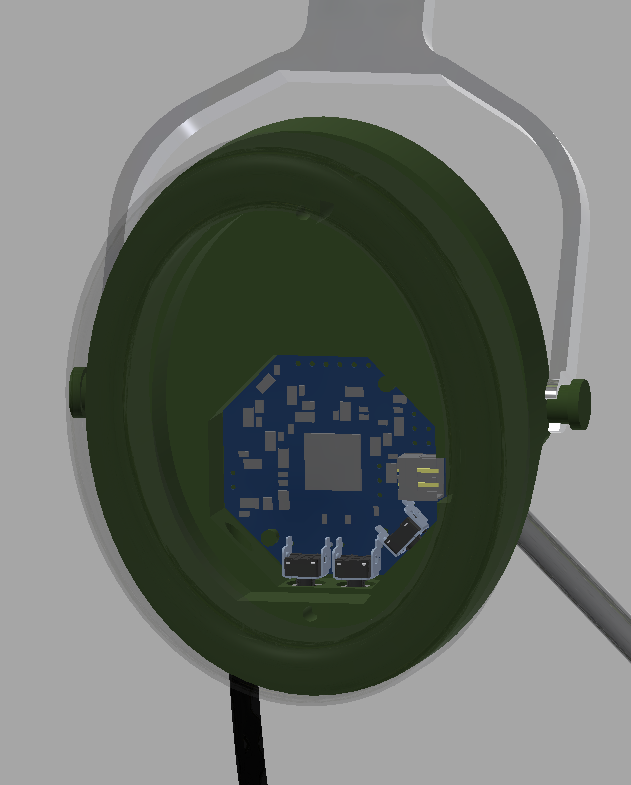
\includegraphics[height=7cm]{zdjecia/model/left_in.png}
		\subcaption{Strona wewnętrzna}
	\end{subfigure}
	\begin{subfigure}{.45\textwidth}
		\centering
		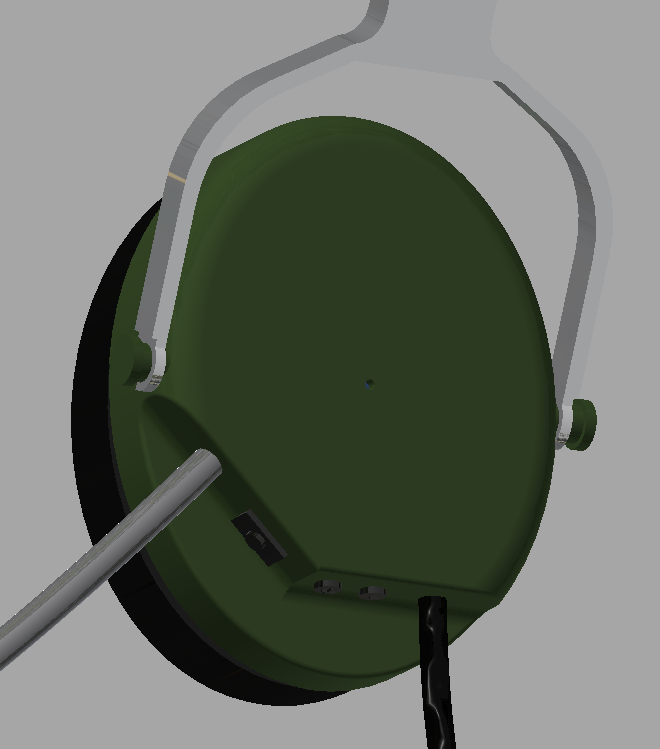
\includegraphics[height=7cm]{zdjecia/model/left_out.png}
		\subcaption{Strona zewnętrzna}
	\end{subfigure}
	\caption{\label{pic:lewa_sluchawka} Model 3D lewej słuchawki}
\end{figure}


\section{Słuchawka prawa}
\label{cha:model_prawa}

Model prawej muszli jest zewnętrznie lustrzanym odbiciem lewej. Różni się otworami na dolnych ściankach wypustu w obudowie. Tutaj zastosowany tylko jeden, pozwalający podłączyć kabel mikro USB. Na zewnętrznej ściance zrobiono dodatkowo niewielki otwór w kształcie baterii, przez który widać światło diody LED, wskazującej stan ładowania słuchawek.

Miejsce na płytkę PCB zostało dostosowane do montażu płytki lewej według wymiarów layoutu i umiejscowione tak, aby port mikrofonu znajdował się na samym środku słuchawki.

\begin{figure}[H]
	\centering
	\begin{subfigure}{.45\textwidth}
		\centering
		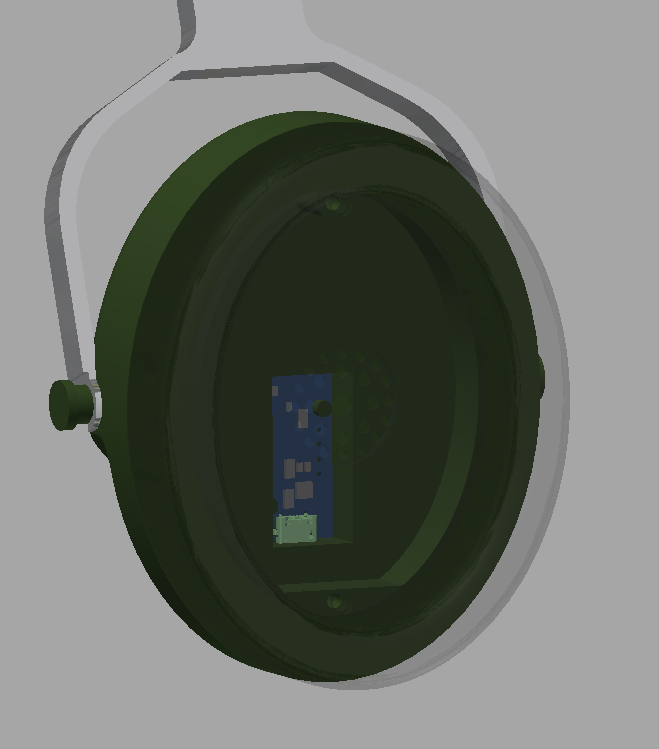
\includegraphics[height=7cm]{zdjecia/model/right_in.png}
		\subcaption{Strona wewnętrzna}
	\end{subfigure}
	\begin{subfigure}{.45\textwidth}
		\centering
		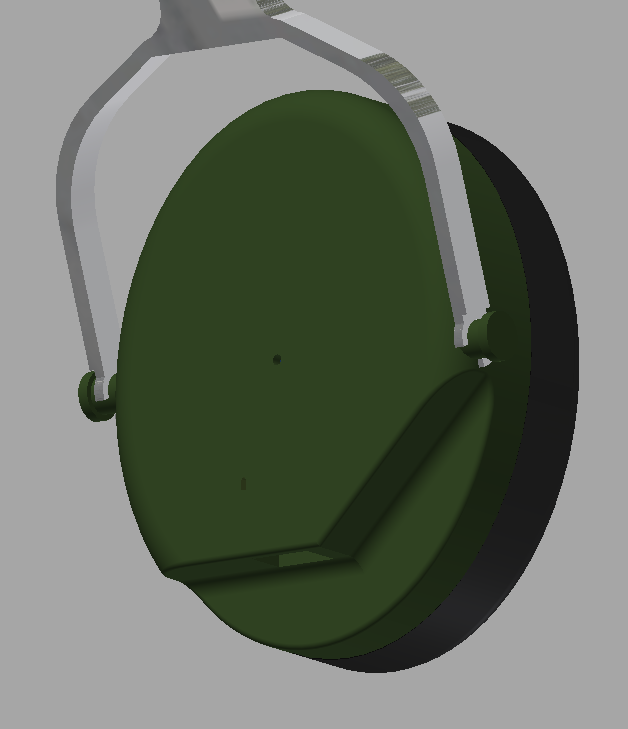
\includegraphics[height=7cm]{zdjecia/model/right_out.png}
		\subcaption{Strona zewnętrzna}
	\end{subfigure}
	\caption{\label{pic:prawa_sluchawka} Model 3D prawej słuchawki}
\end{figure}


\section{Pałąk}
\label{cha:model_palak}

Pałąk słuchawek stworzono na planie okręgu o średnicy $200mm$. Każda ze słuchawek ma dodatkowo własny mały pałąk, który jest montowany na obrotowych zawiasach do muszli oraz wsuwany do głównego pałąku, umożliwiając dostosowanie wysokości do głowy użytkownika.

\begin{figure}[H]
	\centering
	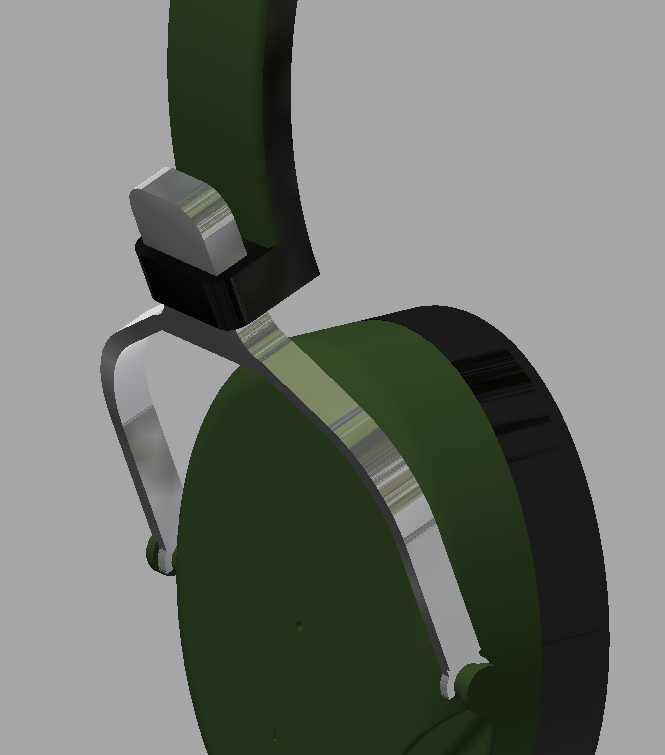
\includegraphics[height=7cm]{zdjecia/model/hinge.png}
	\caption{\label{pic:hinge}Zawias lewej słuchawki}
\end{figure}
	
	\chapter{p o d s u m o w a n k o}
\label{cha:podsumowanie}

Nie działa

Zbudowaliśmy

Tak wygląda:

\begin{figure}[H]
	\centering
	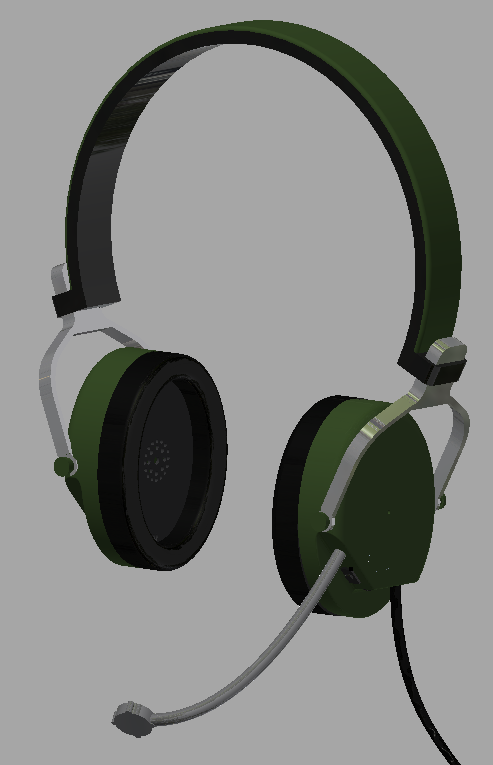
\includegraphics[width=10cm]{zdjecia/model/full_model.png}
	\caption{\label{pic:full_model}Pełna wizualizacja słuchawek}
\end{figure}
	
	\printbibliography
	
\end{document}
